\section{Konzeption und Entwicklung}

\subsection{Grundlagen}
Seit dem Beginn der Entwicklung von Lösungen für VR in den fünfziger Jahren des 20.~Jahrhunderts, gab es stetig neue und innovative Konzepte, um nicht nur mit, sondern auch in der virtuellen Welt zu interagieren~\cite{virtualreality}. In diesem Kapitel wird zunächst erläutert, um was es sich bei VR genau handelt. Danach wird näher auf \textit{head-mounted displays} (HMDs) eingegangen, welche nach dem ersten Prototypen aus dem Jahre 1968 kontinuierlich weiterentwickelt wurden und heute ein vielversprechendes Ein- und Ausgabegerät für Informationen darstellen~\cite{vrfuture}. Daran anschließend folgen grundlegende Erläuterungen zu Eingabegeräten wie \textit{tracking devices}, also Geräten mit Verfolgungssensoren, oder \textit{vision-based devices}, welche abhängig vom Blickwinkel eines Benutzers sind. Die beiden genannten und noch weitere Gerätetypen sind für die Konzeptions-Phase für das zu entwickelnde Interface relevant. Desweiteren werden Details zur Ergonomie aufgeführt, zusammen mit Möglichkeiten und Grenzen durch den menschlichen Körper. Abschließend wird auf \textit{3D user interfaces} (3DUIs) und \textit{body-based interfaces} (BIs) eingegangen, wodurch der Rahmen für das Grundverständnis dieser Arbeit gegeben wird.

\subsubsection{Virtual Reality}
VR erfährt seit der technischen Einführung im Jahre 1968 ein andauerndes Interesse. Das Potenzial von VR entfaltet sich sowohl in der Entwicklung neuer Anwendungen, als auch in der Erforschung neuer Anwendungsgebiete und der Verwendung der bereits vorhandenen Methoden und Mittel im Alltag. Grundlegend ist VR eine interaktive Simulation, bei welcher die menschlichen Sinne verstärkt oder manipuliert werden, um während der Benutzung mit einem Computer, einem Benutzer das Gefühl zu geben, tatsächlich in einer virtuellen Umgebung zu sein~\cite{virtualreality}. Einerseits kann der gesamte Körper des Benutzers in die virtuelle Umgebung übertragen werden, andererseits reicht es teilweise aus, bestimmte Körperteile wie z.B.~die Hände~\cite{handtracking} oder die Finger~\cite{virtualrealityandgames} virtuell abzubilden. Die virtuelle Umgebung besteht dabei aus verschiedenen Objekten, welche untereinander in Beziehung stehen können. Wahrgenommen werden können die platzierten Objekte visuell, auditiv oder haptisch~\cite{virtualreality}. Das bedeutet, dass Objekte entweder der reinen Visualisierung dienen, z.B.~ein Foto in einem Raum, die Akustik unterstützen, z.B.~Windgeräusche, oder Interaktionen zulassen wie z.B.~ein Würfel, welcher geworfen werden kann. Dadurch soll dem Benutzer ein immersives Gefühl und eine sogenannte physische als auch mentale Präsenz vermittelt werden~\cite{hmds}. Physische Präsenz bedeutet, dass der Benutzer das Gefühl bekommt, mit dem eigenen Körper in der virtuellen Welt zu sein. Mentale Präsenz hingegen bedeutet Ansprüche und Erwartungen an die virtuelle Umgebung zu stellen, und somit ein Teilhabe-Gefühl zu entwickeln. Die mentale Präsenz kann dabei unterschiedliche Stadien annehmen. Von einer puren Verbundenheit mit einem Computer, bis hin zum Gefühl, dass die virtuelle Welt real ist. Je nach Anwendungskontext müssen physische und mentale Präsenz einen bestimmten Grad erreichen~\citep{virtualreality}. Dafür notwendig ist das sensorische Feedback. Feedback wird größtenteils visuell vermittelt, z.B.~durch das Einfärben eines Objektes bei einer Selektion. Feedback kann jedoch auch haptisch oder auditiv übertragen werden. Ebenfalls wichtig, ist die Perspektive mit der die virtuelle Umgebung wahrgenommen wird~\cite{virtualreality}. Die Erste-Person Ansicht spiegelt die Sicht eines Menschen in der Realität wider, möglich sind jedoch auch die Zweite-Person Ansicht, sowie die Dritte-Person Ansicht. Letztere auch bekannt als Vogel- oder ISO-Perspektive, dient dem Überblick einer Situation oder Umgebung aus der Ferne~\cite{virtualreality}. Aufgrund des Kontextes dieser Arbeit wird auf Feedback, Perspektiven und Präsenzen nicht weiter eingegangen.\\

\begin{figure}[h]
\captionsetup{width=.7\linewidth}
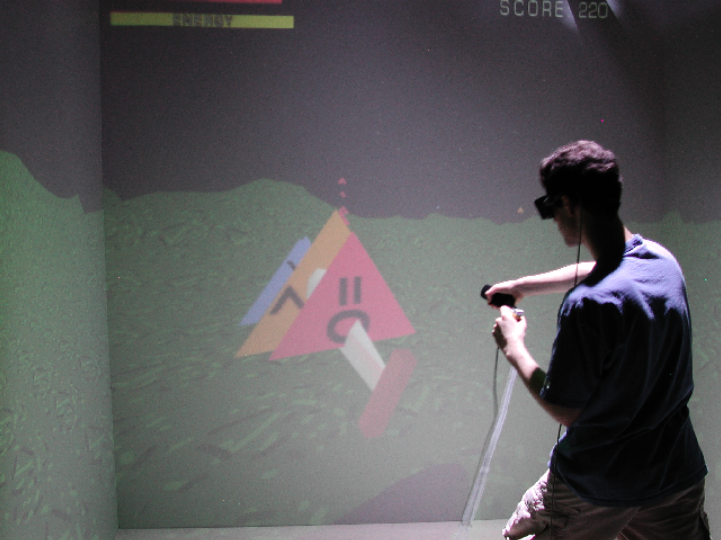
\includegraphics[scale=0.5]{Bilder/Hauptteil/virtualreality}
\centering
\caption{Virtual-Reality Anwendung SwordPlay~\cite{anintroductionto3dspacial}}
\label{fig:vranwendung}
\end{figure}

\subsubsection{Head-mounted displays}
HMDs sind Geräte, welche auf oder an dem Kopf eines Benutzers platziert werden~\cite{hmds}. HMDs unterscheiden sich u.a.~in der Qualität der Auflösung, Farbdarstellung, Sichtfeldweite, Interfacedarstellung sowie Beleuchtung~\cite{hmdsinmedicine}. Aktuelle Geräte wie die Oculus Rift oder HTC Vive, letztere zu sehen in Abbildung \ref{fig:hmds}, verwenden stereoskopische Anzeigen und Aufzeichnungssysteme, um die Kopfbewegungen eines Benutzers zu erfassen und dreidimensionale Bilder darstellen zu können. Um die genaue Position des Kopfes des Benutzers im virtuellen Raum berechnen zu können, kommen Beschleunigungssensoren und Gyroskope zum Einsatz, welche in die HMDs direkt integriert werden~\cite{hmds}.\\

\begin{figure}[h]
\captionsetup{width=.7\linewidth}
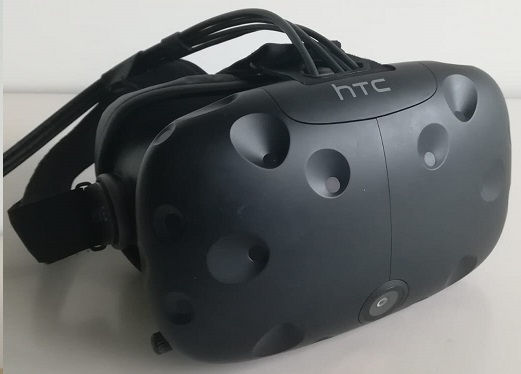
\includegraphics[scale=0.75]{Bilder/Hauptteil/viveheadset}
\centering
\caption{HTC Vive Headset}
\label{fig:hmds}
\end{figure}

\noindent Durch HMDs können u.a.~kognitive, psychomotorische oder affektive Fähigkeiten erlernt und verbessert werden. Unter psychomotorische Fähigkeiten fällt bspw.~die Geschicklichkeit, unter affektive Fähigkeiten die eigenen Gefühle besser kontrollieren zu können. Im Falle von kognitiven Fähigkeiten kann z.B.~das Erinnerungs\-vermögen verbessert werden~\cite{hmdsineducation}. Um eine positive Erfahrung während der Benutzung eines HMDs zu gewährleisten, ist die sogenannte \textit{Field of View} (FOV), also der Sichtradius entscheidend. Der natürliche Sichtradius eines Menschen befindet sich bei 180 Grad. Aktuelle Geräte wie die HTC Vive erreichen eine FOV von über 100 Grad, was sich positiv auf die Erfahrung und dem damit verbundenen Realitätsgefühl auswirkt. Ebenfalls nennenswert ist der Begriff \textit{motion}- bzw. \textit{cybersickness}. Darunter wird ein Übelkeits- oder Schwindelgefühl verstanden, welches bei der Verwendung von HMDs in Verbindung mit VR auftreten kann. \textit{Motionsickness} kann die Immersion beeinträchtigen und dadurch negative Erfahrungen mit HMDs und VR begünstigen. Auch kann \textit{motionsickness} vom Alter, der Erfahrung und des Geschlechts des Benutzers abhängen, was durch diverse Studien nachgewiesen wurde~\cite{hmdsineducation}. Durch die stetige Weiterentwicklung von HMDs, finden die selbigen zunehmend Anwendung in den Bereichen Bildung~\cite{hmdsineducation}, Psychologie~\cite{hmdsinpsychology}, Medizin~\cite{hmdsinmedicine} oder in der 3D-Modellierung~\cite{hmdsinmodeling}.

\subsubsection{Eingabegeräte}
Eingabegeräte sind auch in VR erforderlich, um mit virtuell erstellten Umgebungen interagieren zu können. Je nach Anwendungskontext und Aufgabenstellung können unterschiedliche Eingabegeräte zum Einsatz kommen. 
Nach Ortega et al.~kann jedes Eingabegerät einer vordefinierten Kategorie zugeordnet werden. Ortega et al.~ definieren dazu elf Kategorien und Beschreibungen, auf welche unterschiedlich stark aufgrund der Relevanz zur Arbeit eingegangen wird:\\

\noindent \textit{Keyboard}\\
Tastaturen werden in 3D-Umgebungen z.B.~ für die Navigation oder die Kontrollierung eines Systems, bspw.~das Auslösen von besonderen Aktionen eingesetzt.\\
\\
\noindent \textit{The Mouse and its Decendants}\\
Mäuse und ihre Nachkommen dienen als präzise Eingabegeräte in 3D-Umgebungen. Mäuse können dabei aus mehreren Buttons, sowie einem Rad zum Scrollen und Lichtsensoren für die Erkennung der Mausposition bestehen. Ebenfalls existent sind sogenannte \textit{Trackballs}, bei denen die Positionserkennung über intern verbaute Sensoren und eine bewegliche Kugel zur Interaktion geschieht.\\
\\
\noindent \textit{Joystick and the Gamepad}\\
\textit{Joysticks} und \textit{Gamepads} waren ursprünglich für die Interaktion mit 2D-Umgebungen konzipiert, bspw.~für den Einsatz in einem Flugsimulator. Dabei konnte sowohl in x- als auch in y-Richtung operiert werden. Aktuell sind \textit{Gamepads} mit zwei \textit{Thumbsticks}, also Daumenbuttons, mehreren Schultertasten und Buttons versehen, und sind für 3D-Anwendungen wie z.B.~Videospiele konzipiert. Ein aktuelles Modell ist bspw.~das XBox One \textit{Gamepad}, zu sehen in Abbildung \ref{fig:xboxonegamepad}.\\

\begin{figure}[h]
\captionsetup{width=.7\linewidth}
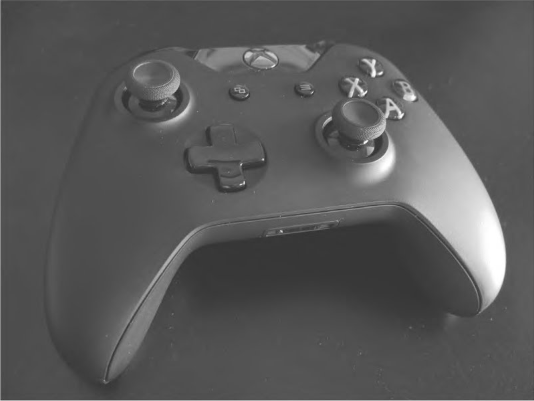
\includegraphics[scale=0.5]{Bilder/Hauptteil/xboxonegamepad}
\centering
\caption{XBox One Gamepad, vgl.~\citep{modernworldinputdevices}}
\label{fig:xboxonegamepad}
\end{figure}

\noindent \textit{3D Mouse and 3D User-Worn Mice}\\
3D-Mäuse bieten im Vergleich zu 2D-Mäusen die Möglichkeit, auch in z-Richtung zu operieren. Dadurch kann z.B.~der Benutzer einer Anwendung durch den virtuellen Raum manövriert oder Objekte bewegt werden. Ein Beispiel für eine 3D-Maus welche am Körper des Benutzers getragen werden kann, ist die als Ring fungierende Maus von Mycestro, zu sehen in Abbildung \ref{fig:mycestro}. Die Maus von Mycestro unterstützt Gestenerkennung, um mit 3D-Anwendungen interagieren zu können.\\

\begin{figure}[h]
\captionsetup{width=.7\linewidth}
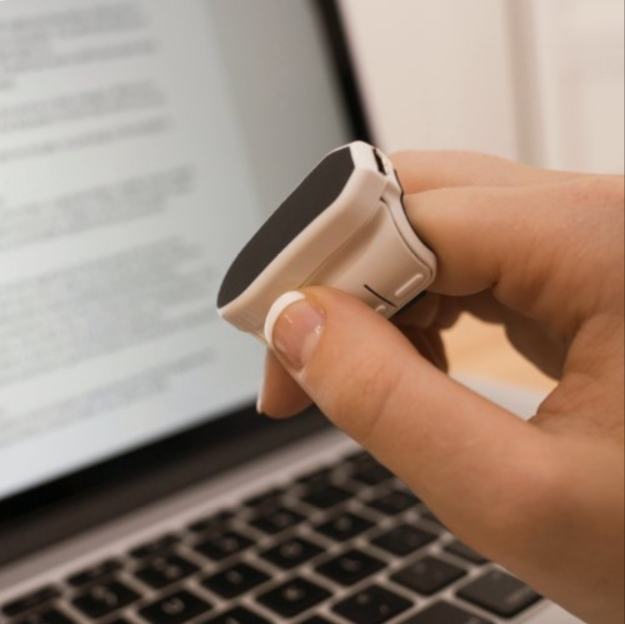
\includegraphics[scale=0.4]{Bilder/Hauptteil/mycestro}
\centering
\caption{Mycestro 3D-Maus Ring, vgl.~\citep{mycestro}}
\label{fig:mycestro}
\end{figure}

\noindent \textit{Audio}\\
Unter Audio als Eingabegerät ist z.B.~ ein Mischpult zu verstehen, welches durch verschiedene auditive Signale, Informationen an einen Computer sendet, welche anschließend verarbeitet werden können.\\
\\
\noindent \textit{Inertial Sensing}\\
Bei \textit{inertial-sensing} werden verschiedene Funktionen durch Druck- bzw.~Trägheitserfassung ausgelöst. Dabei können mehrere Finger bspw.~eine andere Interaktion auslösen, als eine Interaktion mit nur einem Finger. Je nach Druckstärke können Aktionen unterschieden und somit auch 3D-Anwendungen bedient werden. Ein Beispiel wird später in diesem Kapitel aufgeführt.\\
\\
\noindent \textit{Vision-based Devices}\\
Geräte, welche abhängig von dem Blickwinkel und der Umgebung eines Benutzers sind, werden als \textit{vision-based devices} bezeichnet. Dabei können Informationen durch Sensoren und Projektoren in die Umgebung gesendet, oder von der Umgebung empfangen werden.\\
\\
\noindent \textit{Data Gloves}\\
Ein \textit{data glove} ist ein Handschuh, welcher verschiedene Sensoren an Fingern und Handgelenk besitzt, um z.B.~Gesten abzubilden und dadurch mit 3D-Umgebungen interagieren zu können. Dabei können die Geschwindigkeit, Bewegung und Orientierung eines Fingers erfasst und interpretiert werden.\\
\\
\noindent \textit{Psychophysiological Sensing}\\
Psychophysiologische Geräte verarbeiten psychische Informationen wie z.B.~die Hirntätigkeit, und physiologische Informationen wie die Motorik, um daraus Aktionen und Befehle abzulesen. Aufgrund der mangelhaften Relevanz zu dieser Arbeit, wird auf Psychophysiologische Geräte nicht weiter eingegangen.\\
\\
\noindent \textit{Tracking Devices}\\
Unter die \textit{tracking devices}, sprich Geräte die Verfolgungssensoren verbaut haben, fallen u.a.~\textit{finger-tracking}, \textit{hand-tracking}, \textit{head-tracking}, \textit{body-tracking} oder \textit{controller-tracking devices}. Die Verfolgungssensoren erfassen dabei z.B.~Geschwindigkeit, Bewegung und Orientierung des dementsprechenden Körperteils oder Gerätes, und eignen sich somit ebenfalls für den Einsatz in 3D-Umgebungen und 3D-Anwendungen.\\
\\
\noindent \textit{Treadmills as Input Devices}\\
Laufbänder sind Eingabegeräte, welche speziell für die unlimitierte Beweglichkeit in virtuellen Umgebungen konzipiert sind. Der Benutzer eines Laufbandes, wird am Gerät befestigt und durch zusätzliche Ausrüstung wie z.B.~speziell konzipierte Laufschuhe in seiner Bewegung erfasst.
\\
\\
Für diese Arbeit relevant aufgrund der Möglichkeit das Eingabegerät am Körper zu tragen, waren die Kategorien \textit{inertial-sensing}, \textit{data gloves}, \textit{vision-based devices} und \textit{tracking devices}~\cite{modernworldinputdevices}. Als Beispiel für \textit{inertial-sensing} dient das von Harrison et al.~entwickelte System, welches durch Druck durch einen oder mehrere Finger bedient werden kann. Je nach Druckstärke und Druckpunkt, können damit die im System verbauten Vibrationssensoren angeregt und somit unterschiedliche Interaktionen durchgeführt werden~\cite{skinput}. Das von Mistry et al.~entwickelte System SixthSense, dient als Beispiel für ein durch Gesten gesteuertes System in der Kategorie \textit{vision-based devices}. Die am Kopf des Benutzers befestigte Kamera erfasst die Hände und die dargestellten Gesten. Der am Kopf befestigte Projektor wirft Informationen und Interaktionselemente auf Oberflächen aus der Umgebung~\cite{sixthsense}. Ein weiteres Beispiel für ein auf Gesten und Projektoren basierendes System ist LightSpace~\cite{lightspace}. Bei LightSpace kommen jedoch im Vergleich zu SixthSense keine Marker an Fingern oder Umgebung vor. Ein durch einen \textit{data glove} gesteuertes System wurde von Jofre et al.~entwickelt. Der von Jofre et al.~ entwickelte Handschuh besitzt für jeden Finger eigene Sensoren, welche nicht nur die Bewegungen und dessen Geschwindigkeit, sondern auch die Orientierung der Finger und Hand messen und erfassen können. Im Vergleich zu den \textit{vision-based devices}, kommen beim \textit{data glove} keine Projektoren zum Einsatz, da die Informationen direkt vom Handschuh in die an einem Computer laufenden Anwendungen übertragen werden~\cite{dataglove}. Ein System, welches \textit{head-tracking} verwendet, um 3DUIs darzustellen, ist das von Ens et al.~ entwickelte Projekt \textit{the personal cockpit}. Das von Ens et al. entwickelte System, umfasst ein HMD in Form einer Brille und darin verbaute Sensoren. Die verbauten Sensoren erfassen die Richtung in welche der Träger der Brille schaut, und stellt daraufhin verschiedene Interaktionselemente oder Informationen dar~\cite{thepersonalcockpit}. Ein populäres Eingabegerät, welches mit \textit{controller-tracking}, VR und HMDs in Verbindung gesetzt wird, ist z.B.~der HTC Vive Controller, zu sehen in Abbildung \ref{fig:vivecontroller}.

\begin{figure}[h]
\captionsetup{width=.7\linewidth}
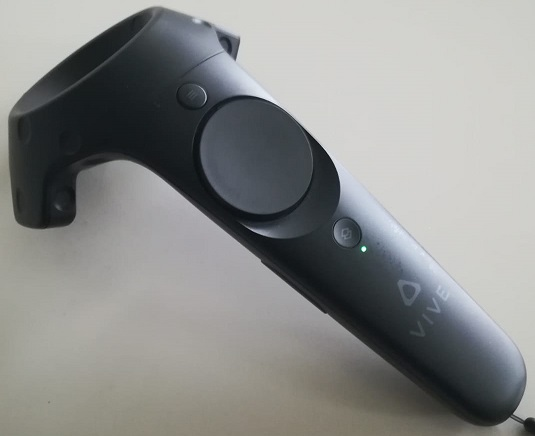
\includegraphics[scale=0.6]{Bilder/Hauptteil/vivecontroller}
\centering
\caption{HTC Vive Controller}
\label{fig:vivecontroller}
\end{figure}

Durch sogenannte \textit{Positioner}, welche im Raum um den Benutzer herum platziert werden, werden nicht nur die Position und Rotation der Controller, sondern wenn gewünscht der gesamte Körper eines Benutzers erfasst. Knöpfe und Touchpads dienen als Eingabemechanismen und können zusammen mit Bewegung und Rotation der Controller sogar Gesten abbilden und so mit einer 3D-Umgebung interagieren~\cite{wearablehtcvive}. Als Beispiel für eine \textit{Treadmill}, also ein Laufband zur Eingabe von Informationen, dient der Virtualizer von Cyberith. Der Benutzer wird dabei in der Mitte des Gerätes befestigt. Die Bewegungen des Benutzers werden durch speziell konzipierte Laufschuhe erfasst und in Interaktionen umgesetzt~\citep{virtualizer}. Aufgrund der zahlreichen Einsatzmöglichkeiten, der speziell für VR entwickelten Hardware, Gestenerkennung und \textit{body-tracking}, sowie der unmittelbaren Verfügbarkeit, bieten sich die HTC Vive Controller in Kombination mit dem HTC Vive Headset für diese Arbeit am Besten an. Tabelle \ref{tab:eingabesysteme} listet die beschriebenen Eingabearten und dazugehörigen Systeme zusammengefasst auf.

%\begin{table}[h]
%\begin{center}
%	\begin{tabular}{| l | l |}
%	\hline
%		\multicolumn{1}{|c|}{\textbf{Eingabeart}} & \multicolumn{1}{|c|}{\textbf{Beispielsystem}} \\[0.3cm] \hline
%		\textit{inertial-sensing} & Skinput \\ \hline
%		\textit{data gloves} & DG5 Vhand Data Glove 2.0 \\ \hline
%		\textit{vision-based devices} & SixthSense, LightSpace \\ \hline
%		\textit{tracking devices} & The personal cockpit, HTC vive controller \\ \hline
%	\end{tabular}
%	\caption{Eingabearten und Systeme}
%	\label{tab:eingabesysteme}
%\end{center}
%\end{table}

\begin{table}[h!]
\begin{center}
  \begin{tabular}{ | c | c | c | }
    \hline
    \textit{Inertial Sensing} & \textit{Vision-based Devices} & \textit{Data Glove} \\ 
    \hline
    \begin{minipage}{.3\textwidth}
    \vspace*{0.1cm}
      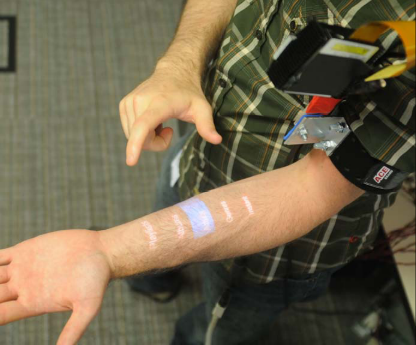
\includegraphics[scale=0.4]{Bilder/Hauptteil/skinput}
    \vspace*{0.1cm}
    \end{minipage}
    &
    \begin{minipage}{.3\textwidth}
      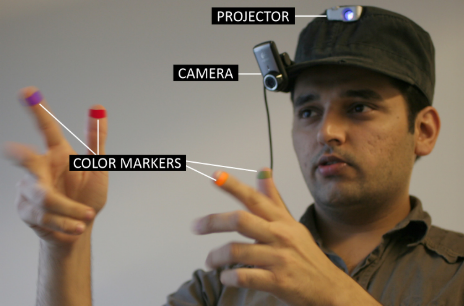
\includegraphics[scale=0.4]{Bilder/Hauptteil/sixthsense}
    \end{minipage}
    &
    \begin{minipage}{.3\textwidth}
    \vspace*{0.1cm}
      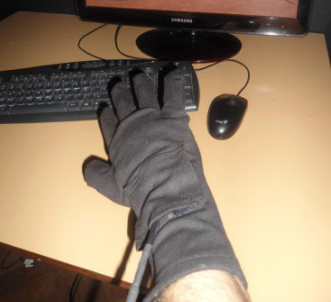
\includegraphics[scale=0.45]{Bilder/Hauptteil/dataglove}
    \vspace*{0.1cm}
    \end{minipage}
    \\ 
    \hline
    Skinput & SixthSense & Data glove \\
    \hline
    \textit{Head-tracking} & \textit{Controller-tracking} & \textit{Treadmill} \\
    \hline
    \begin{minipage}{.3\textwidth}
      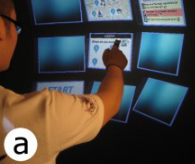
\includegraphics[scale=0.8]{Bilder/Hauptteil/thepersonalcockpit}
    \end{minipage}
    &
    \begin{minipage}{.3\textwidth}
      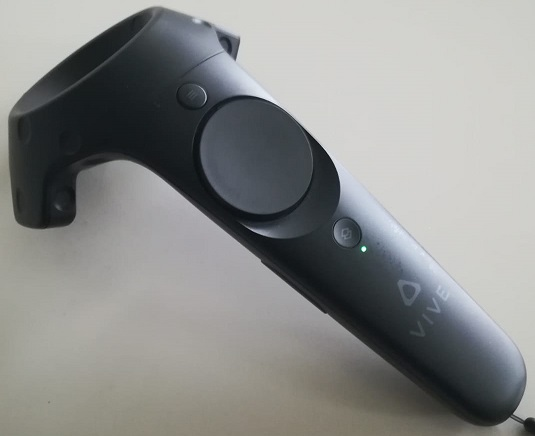
\includegraphics[scale=0.3]{Bilder/Hauptteil/vivecontroller}
    \end{minipage}
    &
    \begin{minipage}{.3\textwidth}
    \vspace*{0.1cm}
      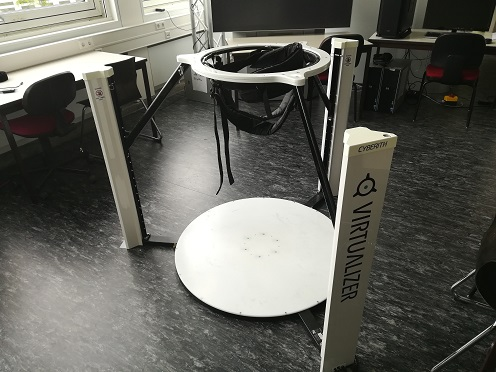
\includegraphics[scale=0.3]{Bilder/Hauptteil/virtualizer1}
    \vspace*{0.1cm}
    \end{minipage}
    \\ 
    \hline
    \textit{The personal cockpit} & \textit{ HTC Vive Controller} & \textit{Cyberith Virtualizer} \\
    \hline
  \end{tabular}
  \caption{Eingabearten und Systeme}
  \label{tab:eingabesysteme}
\end{center}
\end{table}

\subsubsection{Ergonomie}
Ergonomie bedeutet im Kontext dieser Arbeit, die Nützlichkeit eines Interfaces zur Erreichung einer Aufgabe, sowie die Benutzungsfreundlichkeit während der Verwendung eines Interfaces. Ein Interface soll, wenn es ergonomisch entwickelt wird, einem Benutzer helfen, eine Aufgabe einfach, effektiv und mit wenig Aufwand durchführen zu können~\citep{ergonomics}. Um z.B.~mit virtuellen Objekten oder Umgebungen interagieren zu können, werden u.a.~Interfaces benötigt, welche je nach Anwendung unterschiedlich in die 3D-Umgebung eingebunden werden. Dabei sollten nicht nur die Art der Interaktionen, sondern u.a.~auch der menschliche Körper mit seinen ergonomischen Möglichkeiten und Limitierungen berücksichtigt werden.
Nur somit ist es möglich, Interfaces zu entwickeln, welche komfortabel und effektiv genutzt werden können. Unterschiedliche Interaktionen erfordern unterschiedliche Bewegungen, welche wiederum unterschiedlich komplex und andauernd sein können. Die Interaktionen haben dabei verschieden stark ausgeprägte Attribute wie Genauigkeit, Geschwindigkeit, Richtung und Dauer. Aufgrund der menschlichen Physiologie können bestimmte Interaktionen län\-ger und präziser oder nur bedingt und umständlich umgesetzt werden, was bei der Implementierung von 3DUIs in VR zu beachten ist~\cite{theoryandpracticebook}. Die menschliche Hand z.B.~bietet durch ihre praktikable Ergonomie eine umfangreiche Palette an Einsatzmöglichkeiten. Darunter das Greifen oder Halten eines Gegenstandes, oder die Möglichkeit Gesten und Posen darzustellen. Ein unangenehmes Maß an Kraft, Dauer und Wiederholung einer Aufgabe, kann sich negativ auf die Erfahrung mit einem System auswirken, gleich wie gut ein Interface entwickelt wurde. Ein weiterer wichtiger Aspekt in der Gestaltung von 3DUIs unter Berücksichtigung der Ergonomie des Menschen, ist das sogenannte \textit{Gorilla arm syndrome}. Darunter wird das Ermüden der Arme durch lang andauernde und unbequeme Posen verstanden. Interfaces, welche auf Augenhöhe oder sogar darüber platziert sind, begünstigen den Gorilla-Arm Effekt. Darum sollten Interfaces möglichst niedrig gehalten oder Interaktionen näher an den Körper gebracht werden. Das Greifen eines weit entfernten Objektes könnte bspw.~durch eine Pointer-Technik ermöglicht werden, um das Ausstrecken des Armes zu vermeiden~\cite{theoryandpracticebook,consumedindurance}. Ein weiteres Anzeichen für Ermüdung ist ein Haltungswechsel. Deshalb sollten Posen bevorzugt werden, welche komfortabel und energiesparend durchgeführt werden können und somit, die Bequemlich- und Leichtigkeit unterstützen. Interfaces, welche sich am Arm oder auf der Hand befinden, haben dabei in Studien großen Zuspruch gefunden, da sich Arm- bzw.~Handinterfaces ergonomisch günstig anbieten und viel Raum als auch Möglichkeiten für Interaktionen bieten~\cite{implicationsoflocation}.
Komfort ist jedoch nicht gewährleistet unter reiner Berücksichtigung der aufgeführten Aspekte. Komfort ist ebenfalls bedingt, durch die Darstellung der Interfaces, bezogen auf Form und Gestalt~\cite{theoryandpracticebook}.

\subsubsection{3D Benutzungsoberflächen}
3DUIs erfahren seit der Alltagstauglichkeit von VR stetig wachsenden Zuspruch und Anwendung. 3DUIs unterscheiden sich in erster Linie von zweidimensionalen UIs durch die gegebenen \textit{degree of freedom} (DOF)~\cite{whatuserinterfacetouse,asurveyon3dobjectmanipulation,theoryandpracticebook}. Die DOF geben an, inwieweit in einer virtuellen Umgebung mit virtuellen Objekten interagiert werden kann, bzw.~wie stark die Operationsvielfalt im virtuellen Raum ausgeprägt ist. Bei 2DUIs beschränkt sich die Interaktion auf Operationen in x und y Richtung. Das bedeutet, dass 2DUIs wie z.B.~ein Dateimanager und dessen Elemente nur in der x und y Richtung positioniert werden können~\cite{issuesandbenefitsofusing3d}. Bei 3DUIs hingegen kommt die Tiefe durch die z-Achse hinzu, wodurch sowohl dreidimensionale Manipulation als auch Rotation ermöglicht werden~\cite{anintroductionto3dspacial}. Die dazugekommene Tiefe kann jedoch auch zu höheren Fehlerraten in der Ausführung von Aufgaben führen, bspw.~beim Selektieren eines Objektes, welches sich dicht neben und kaum hinter einem anderen Objekt befindet. Die Bevorzugung von 3DUIs gegenüber 2DUIs hängt demnach von der Anwendung und dessen Kontext ab. Kyritsis et al.~haben bspw.~nachgewiesen, dass sich ein 3D-Dateimanager, aufgezeigt in Abbildung \ref{fig:3dinterface}, in Verbindung mit VR nur anbietet, wenn die Darstellung der Dateien durch große und auffällig eingefärbte Symbole gegeben ist~\cite{issuesandbenefitsofusing3d}.

\begin{figure}[h]
\captionsetup{width=.7\linewidth}
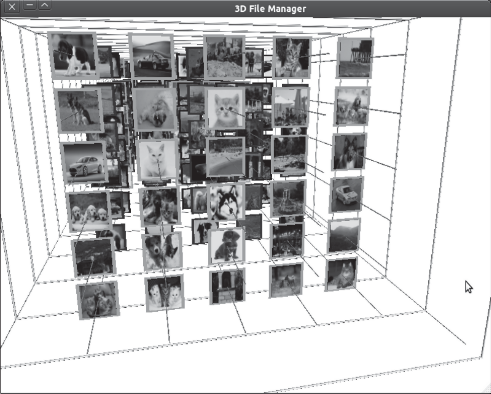
\includegraphics[scale=0.75]{Bilder/Hauptteil/3duserinterface}
\centering
\caption{3D Dateimanager~\cite[p.~243]{issuesandbenefitsofusing3d}}
\label{fig:3dinterface}
\end{figure}

\noindent Eine Eigenschaft die 3DUIs gegenüber 2DUIs mit sich bringen, ist die Vielfalt der Darstellung und Interaktion. So können 3DUIs bspw.~frei in der virtuellen Umgebung platziert~\cite{anintroductionto3dspacial}, und/oder durch Gesten~\cite{introduction3dgesturalinterfaces} gesteuert werden. Die Komplexität von 3DUIs reicht von Interfaces welche sich bei Kopfdrehungen während des Tragens eines HMD mit bewegen, um die Position des 3DUI zu ändern, bis hin zu komplexen Modellierungs- oder Designinteraktionen. Mike Alger hat zahlreiche Prototypen mit unterschiedlichen Anwendungszwecken entwickelt, welche den Nutzen von 3DUIs in VR bei Verwendung eines HMD verdeutlichen~\citep{mikealger}. Abbildung \ref{fig:mikealger} zeigt einen dieser Prototypen, bei welchem die Verwaltung und Interaktion mit Dokumenten im Vordergrund steht.

\begin{figure}[h]
\captionsetup{width=.7\linewidth}
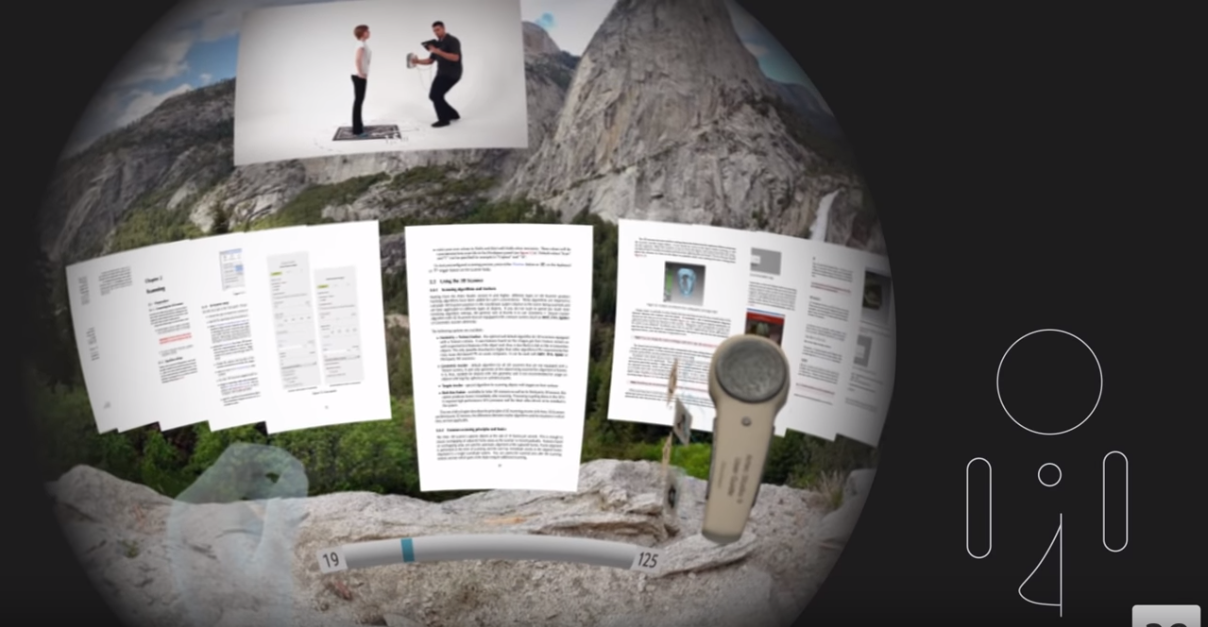
\includegraphics[scale=0.3]{Bilder/Hauptteil/mikealger3dui}
\centering
\caption{3DUI Prototyp für VR bei Verwendung eines HMD, vgl.~\citep{mikealger}}
\label{fig:mikealger}
\end{figure}

\noindent Eingesetzt werden 3DUIs u.a.~auch in den Bereichen Videospiele, Unterhaltung, Simulation, Bildung oder der Medizin~\cite{theoryandpracticebook}. Da sich 3DUIs so unterschiedlich komplex und vielfältig im Design ausprägen können, wirken sich die selbigen auch unterschiedlich auf die \textit{user experience} (UX), also die Erfahrung, welche Benutzer bei Verwenden eines Interfaces erlangen, aus~\citep{constraints3duis}. Um eine einfache und positive Nutzung von 3DUIs sicherstellen zu können, haben Burmester et al.~ bspw.~Interaktionsmuster definiert, welche einen Standard in der Entwicklung von dreidimensionalen Interfaces, u.a.~auch für VR-Anwendungen bieten sollen. Die definierten Interaktionsmuster sind weiterhin in Entwicklung und werden an technologische Gegebenheiten und Neuerungen wenn nötig angepasst~\cite{interactionpatterns}.

\subsubsection{Körperbasierte Interfaces}
Body-based Interfaces (BIs) versuchen sowohl die Ein- als auch die Ausgabe von Informationen über den menschlichen Körper zu bewerkstelligen~\cite{implicationsoflocation}. Das Ziel ist, den menschlichen Körper so zu instrumentalisieren, sodass keine externen Geräte mehr wie z.B.~Smartphones benötigt werden, um Daten verarbeiten, Anwendungen nutzen oder mit anderen Menschen global kommunizieren zu können~\cite{skinput}. Berücksichtigt werden sollte dabei nicht nur die Ergonomie, sondern auch die Nutzergruppe, für die ein BI entwickelt wird. Harrison and Faste haben dazu herausgefunden, dass bestimmte Positionen für körperbasierte Interfaces von Frauen und Männern unterschiedlich streng empfunden wurden. Für die anwesenden Frauen z.B.~, war ein Interface im Schulter- oder Oberarmbereich unvorstellbar, da es zu privat oder unangenehm wäre. Allgemein akzeptabel und angenehm, war bei dem Experiment wiederum der Unterarm- und Handbereich~\cite{implicationsoflocation}. Durch die emotionale Verbundenheit zum eigenen Körper ist es möglich, verschiedenste Arten von körperbasierten Interfaces anzuwenden und zu entwickeln. Die Vielfältigkeit zeigt sich anhand der folgenden Beispiele. Skinput ist ein BI, welches die durch den Körper geleiteten Impulse eines Fingerschlages aufzeichnet und interpretiert. Je nach Stärke und Dauer eines Impulses, können unterschiedliche Aktionen durchgeführt werden~\cite{skinput}. OmniTouch von Harrison et al., zu sehen in Abbildung \ref{fig:omnitouch}, nutzt eine Microsoft Kinect als Tiefenkamera sowie einen Projektor welche auf der Schulter des Benutzers befestigt werden, um Interfaces ausgehend von der Position des Trägers, beliebig auf Hände und Arme zu projizieren. Die Finger des Trägers werden dabei aufgezeichnet. Durch Gesten oder simple Berührungen auf dem BI können Benutzer z.B.~Objekte skalieren oder zeichnen~\cite{omnitouch}.\\

\begin{figure}[h]
\captionsetup{width=.7\linewidth}
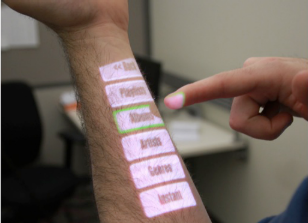
\includegraphics[scale=1]{Bilder/Hauptteil/onbodyinterface}
\centering
\caption{Anwendung von OmniTouch~\cite[p.~446]{omnitouch}}
\label{fig:omnitouch}
\end{figure}

\noindent Ein weiteres Beispiel stellt PalmRC dar. Bei PalmRC wird die Handfläche eines Menschen zum Eingabegerät für Aktionen mit einem TV-Gerät. Die Handfläche besitzt dabei imaginäre Markierungen, an die diverse Funktionen gekoppelt sind, bspw.~das Umschalten eines Programmes oder das Hoch- und Runterscrollen durch die Senderliste~\cite{palmrc}. BIs haben durch die Verbundenheit zum eigenen Körper den Vorteil, leicht bedienbar und einprägsam zu sein. Ein statisches Interface kann somit einfach erlernt und sogar mit geschlossenen Augen und ausreichender Übung bedient werden~\cite{implicationsoflocation}.

\subsubsection{Anforderungen aus Grundlagen}
Aus den aufgeführten Fakten der vorhergegangenen Kapitel, erschließen sich die Anforderungen aufgelistet in Tabelle \ref{tab:grundlagenanforderungen}, welche beim Design- und Entwicklungsprozess zusätzlich berücksichtigt werden.

\begin{table}[h]
\begin{center}
  \begin{tabular}{| p{11cm} |}
    \hline
     \makecell[l]{Sensorisches Feedback für Aktionen wie Selektion bieten}\\ \hline
     \makecell[l]{Zweihändige Gesten vermeiden}\\ \hline
     \makecell[l]{Interface auf Unterarm oder Hand platzieren}\\ \hline
     \makecell[l]{Ruheposen zur Erholung bereitstellen}\\ \hline
     \makecell[l]{Interaktionsmuster in Designphase berücksichtigen}\\
     \hline
  \end{tabular}
  \caption{Anforderungen aus vorangegangenen Kapiteln}
	\label{tab:grundlagenanforderungen}
\end{center}
\end{table}

\subsection{Hinführung zum Konzept}
In diesem Kapitel wird näher auf die Aspekte eingegangen, welche sowohl für die Entwicklung der Anwendung als auch für das Interface relevant sind. Zunächst folgen Anforderungen, welche sowohl für das Interface als auch für die Anwendung gestellt werden. Anschließend werden Richtlinien aufgelistet, welche bei der Entwicklung des Interfaces berücksichtigt werden. Danach folgt ein Abschnitt über die Wahl der Position des Interfaces. Dabei wird näher darauf eingegangen, welche Vorteile der menschliche Arm mit sich bringt, und warum sich speziell der Unterarm im Kontext dieser Arbeit als beste Wahl für ein Interface anbietet. Im Anschluss daran folgen Konzepte von bereits etablierten Designs, sowie Beschreibungen, weshalb ein Design für eine Anwendung mit Modellierungsansatz und körperbasierter Eingabe in VR geeignet oder nicht geeignet ist. Abschließend wird das finale Konzept für den Prototypen aufgezeigt und beschrieben.

\subsubsection{Anwendungsanforderungen}
Aus dem Kontext der Arbeit, den aufgeführten ergonomischen Einschränkun\-gen und dem Austausch mit Experten des Fraunhofer IAO in Stuttgart, sind Anforderungen für die zu entwickelnde Anwendung entstanden, welche in Tabelle \ref{tab:anwendungsanforderungen} aufgelistet sind.
\begin{table}[h]
\begin{center}
  \begin{tabular}{| P{1cm} | p{12cm} |}
    \hline
     1. & \makecell[l]{Primitive Körper wie Würfel und Kugeln können erstellt \\ und gelöscht werden}\\ \hline
     2. & Einzelne Objekte sind selektierbar\\ \hline
     3. & \makecell[l]{Erstellte Objekte können in Position, Rotation \\ und Größe manipuliert werden}\\
    \hline
    4. & \makecell[l]{Der Benutzer bekommt Informationen zur \\ Benutzung von Funktionen}\\
    \hline
    5. & \makecell[l]{Die Rotation und Translation eines selektierten Objektes \\ ist durch eine einhändige Geste möglich}\\
    \hline
    6. & Selektierte Objekte können deselektiert werden \\
    \hline
    7. & Die Anwendung kann vom Benutzer beendet werden\\
    \hline
  \end{tabular}
  \caption{Anwendungsanforderungen}
	\label{tab:anwendungsanforderungen}
\end{center}
\end{table}

\subsubsection{Richtlinien}
Bei der Entwicklung von 3DUIs können diverse Richtlinien und Vorgaben beachtet werden, welche für eine positive UX bei der Verwendung des zu entwickelnden Interfaces sorgen sollen~\citep{interactionpatterns}. Die Richtlinien und Vorgaben beziehen sich dabei u.a.~auf ergonomische Gegebenheiten, als auch auf technische und andere äußere Faktoren. Ein wichtiger Punkt für die Verwendung von Interfaces durch Gesten und Touch, ist die Komplexität und Natürlichkeit der Interaktionen~\cite{asurveyon3dobjectmanipulation}. Funktionen wie Selektion oder Objektmanipulation sollten einfach und natürlich gestaltet sein. Das Greifen eines Objektes in der Realität kann z.B.~demnach exakt in VR nachgestellt werden, um die Immersion zu erhöhen. Ebenfalls sollten die DOF so weit wie möglich, wenn möglich, reduziert werden, um die Fehlerrate zu verringern und einer Überforderung vorzubeugen. Auch \textit{bi-manual interactions}, also zweihändige Interaktionen, sollten aufgrund der eventuellen Komplexität vermieden werden, da dadurch der Gorilla-Arm Effekt, in Kapitel 2.1.4 bereits erläutert, gefördert wird~\cite{asurveyon3dobjectmanipulation}. Funktionen, welche auf dem Arm der nicht dominierenden Hand platziert werden, sollten nach Stuerzlinger und Wingrave so angebracht werden, sodass andere Funktionen weder geschnitten noch überlagert werden~\cite{constraints3duis}. Auch sollten nach Stuerzlinger et al.~schwebende Objekte an andere Objekte befestigt werden, sodass ein natürliches Gefühl für die Elemente entsteht. Für die Selektion und Manipulation von Objekten im virtuellen Raum, sollte außerdem die Überdeckung und Tiefenwahrnehmung berücksichtigt werden. Objekte welche so weit vom Benutzer entfernt sind, sodass ein simples Greifen nicht mehr ausreicht, sollten durch Techniken wie Pointer oder \textit{ray-casting} selektier- und manipulierbar gemacht werden~\cite{anintroductionto3dspacial}. Für die Rotation von Objekten, bedarf es einer Lösung, welche das Handgelenk kaum belastet und die Ergonomie des selbigen berücksichtigt. Ebenso wichtig ist die Entfernung von Funktionen und Interaktionsmöglichkeiten vom Benutzer zum Interface. Weit entfernte Elemente verursachen Zittern und Ungenauigkeit, wodurch die Fehlerrate erhöht und eine negative Erfahrung in der Benutzung mit dem Interface und der Anwendung erlangt wird~\cite{anintroductionto3dspacial}. Desweiteren sollten nach Riecke et al.~klammernde oder packende Gesten vermieden und eher auf einhändige, simple Gesten gesetzt werden~\cite{virtualrealityandgames}. Jedoch gilt es nicht nur das Interface und die Interaktionen so einfach wie möglich zu halten, sondern auch die Umgebung. Wichtig hierbei ist das Feedback bei der Verwendung von 3DUIs~\cite{theoryandpracticebook}. Das temporäre und dreidimensionale Feedback sollten dabei übereinstimmend sein, sprich die Bewegungen des Benutzers in der virtuellen Umgebung sind auf die natürlichen Bewegungen des Benutzers in der Realität abgestimmt, um ein positives Nutzererlebnis herzustellen und aufrechtzuerhalten. Zusätzlich in Betracht gezogen werden kann die Textur und der Stil des Interfaces. Je echter und hochwertiger das Interface gestaltet ist, desto mehr wird von der Interaktion und der Anwendung erwartet. Ein gezeichneter oder Karikatur ähnlicher Stil ist bei simplen Anwendungen zu bevorzugen, da sowohl das Erlernen als auch das Verstehen des Interfaces dadurch erleichtert wird~\cite{theoryandpracticebook}.

\subsubsection{Interfacepositionierung}
Die Position eines Interfaces ist mitunter ausschlaggebend, ob eine Anwendung komfortabel und praktisch benutzt werden kann. Aufgrund der be\-reits beschriebenen ergonomischen Gegebenheiten und dem Hintergrund, dass das Interface in einem Modellierungskontext verwendet werden soll, konn\-ten diverse Positionen und Umsetzungen von vornherein ausgeschlossen werden. Die zusätzliche Dimension, welche durch 3D hinzu kommt, bringt zwar Probleme wie Überdeckung oder falsche Tiefeneinschätzung mit sich, wirkt sich jedoch positiv auf die Immersion aus und bietet gerade aufgrund der zusätzlichen Tiefe, neue Möglichkeiten für Interaktionen~\cite{constraints3duis}. Die Arme haben sich als praktisches Mittel in der Arbeit mit VR erwiesen, da durch die horizontale Ausdehnung genügend Platz für diverse Funktionen vorhanden ist~\cite{skinput}. Außerdem sind Arme gut beweglich und benötigen keine unbequemen Bewegungen um anvisiert werden zu können, was während der Benutzung eines HMD aufgrund der eingeschränkten FOV wichtig ist. Auch aufgrund von zweihändigen Funktionen, bietet sich der Unterarm für ein Interface an. Die nicht dominierende Hand kann dabei die Funktionen visualisieren, während die andere Hand die Funktionen selektiert und verwendet. Die Präzision wird durch die körperbasierte Lösung ebenfalls erhöht, da das Ausstrecken und Heben der Arme, um mit einem Interface interagieren zu können, nicht mehr notwendig ist. Zittern und Verzerrung, was zu ungenauen Eingaben führt, sowie die Ermüdung der Arme fällt damit weg~\cite{theoryandpracticebook,anintroductionto3dspacial,consumedindurance}. Auch kann das körperbasierte Interface durch die Nähe zum eigenen Körper, recht große und eindeutige Elemente enthalten, welche die Menünavigation erleichtern können~\cite{constraints3duis}. Desweiteren können durch das Arm-Interface die dazugehörigen Elemente so platziert werden, dass kein Element ein anderes überdeckt. Aktivierte Funktionen blenden nicht benötigte Funktionen aus, oder erweitern ihren Kontext durch Anordnung der Unterlemente in andere Richtungen, sodass andere Funktionen sichtbar bleiben~\cite{implicationsoflocation}.
Aufgrunddessen dass in der Rea\-lität fliegende oder schwebende Objekte an einem anderen Objekt befestigt sind, bieten sich die Arme als Interfaceposition an, da somit eine Immersion der Verbindung zur Hand und zum eigenen Körper aufgebaut wird~\cite{constraints3duis}.
Durch die Verbindung zum eigenen Körper ist es durchaus möglich, nach einer gewissen Zeit an Übung, das Interface auch blind bedienen zu können~\cite{theoryandpracticebook}.

\subsubsection{Verwandte Ideen und Konzepte}
Die folgenden Designideen für das Interface unterscheiden sich sowohl in Form als auch in Komplexität, auf welche jeweils eingegangen wird. Für diese Arbeit war es wichtig, ein Interface zu entwickeln, welches durch direkte Eingabemechanismen wie Touch bedient werden kann. Somit konnten Ansätze für Pointer-Techniken in der Designphase ausgeschlossen werden.

\subsubsection*{3D Wheel picker}
\noindent Die erste Idee war ein nach Ehrlich sogenannter \textit{wheelpicker}, zu sehen in Abbildung \ref{fig:wheelpicker1}. Beim \textit{wheelpicker} werden die verfügbaren Interaktionen auf einem Wheel, sprich einem runden Körper platziert. Der \textit{wheelpicker} kann beliebig breit gestaltet werden. Die Funktionen können durch eine simple Rotation des Armes visualisiert oder auch je nach Winkel und gewünschter Funktionalität deaktiviert werden~\cite{wheelpickerpiemenu}.

\begin{figure}[h]
\captionsetup{width=.7\linewidth}
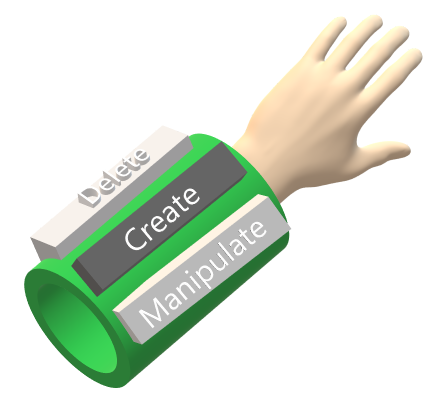
\includegraphics[scale=0.5]{Bilder/Hauptteil/konzept8}
\centering
\caption{Wheelpicker-Modell nach~\cite[p.~33]{wheelpickerpiemenu}}
\label{fig:wheelpicker1}
\end{figure}

\noindent Nachteil des Wheelpicker-Ansatzes ist jedoch die Bedienung. Das blinde Bedienen des \textit{wheelpicker} wird durch die zusätzlich benötigte Rotation des  Armes erschwert. Der Ansatz des Deaktivierens von Funktionen welche nicht im korrekten Winkel liegen, kann die blinde Bedienung zusätzlich erschweren. Auch kann die Nichtsichtbarkeit von Bedienelementen aufgrund der Rotation des Armes die Bedienung erschweren~\cite{theoryandpracticebook}. Ebenfalls kann es aufgrund der Anbringung der Funktionen zu Überdeckungen während der Bedienung kommen, zu sehen in Abbildung \ref{fig:wheelpicker2}.

\begin{figure}[h]
\captionsetup{width=.7\linewidth}
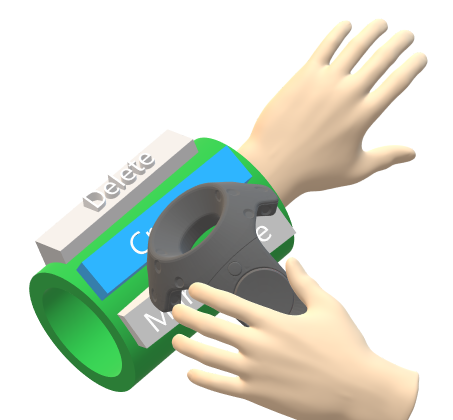
\includegraphics[scale=0.5]{Bilder/Hauptteil/konzept9}
\centering
\caption{Interaktion mit Wheelpicker-Modell nach~\cite[p.~33]{wheelpickerpiemenu}}
\label{fig:wheelpicker2}
\end{figure}

\subsubsection*{Pie menu}
\noindent Eine weitere Idee war ein an von LaViola et al.~angelehntes \textit{radial-} bzw.~sogenanntes \textit{pie menu}, visualisiert in Abbildung \ref{fig:piemenu1}. Das \textit{pie menu} ist ein kreisförmiges Interface, bei dem die Elemente in gleichmäßigen Abständen nebeneinander platziert werden. Das \textit{pie menu} ist im Vergleich zum \textit{wheelpicker} ein 2D-Modell und bietet dadurch keine Tiefe~\cite{theoryandpracticebook}.

\begin{figure}[h]
\captionsetup{width=.7\linewidth}
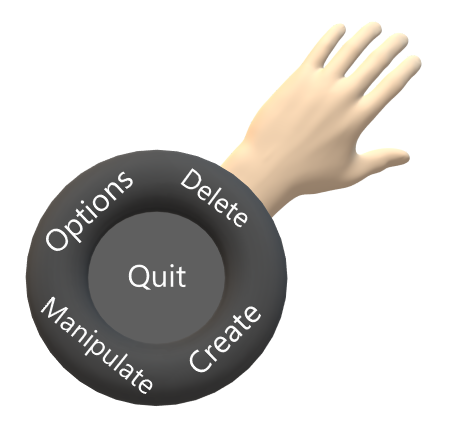
\includegraphics[scale=0.5]{Bilder/Hauptteil/konzept10}
\centering
\caption{Pie-Modell nach~\cite[p.~10]{wheelpickerpiemenu}}
\label{fig:piemenu1}
\end{figure}

\noindent Beim \textit{pie menu} wird auch keine Rotation benötigt, um versteckte Funktionen sichtbar zu machen. Somit wird das Erlernen des Interfaces und die damit verbundene blinde Bedienung gegenüber dem \textit{wheelpicker} erleichtert. Nachteil des \textit{pie menu} ist wiederum die Überdeckung sowie die Anbringung der Elemente auf unterschiedlicher Höhe und Breite, was eine erhöhte Lernkurve zur Folge hat.

\begin{figure}[h]
\captionsetup{width=.7\linewidth}
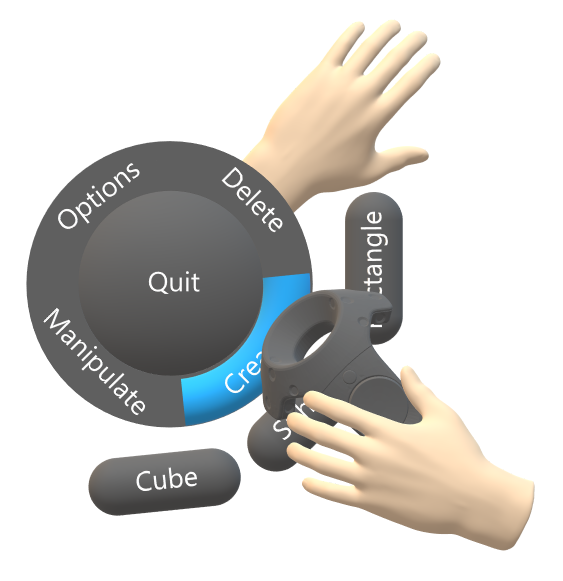
\includegraphics[scale=0.5]{Bilder/Hauptteil/konzept11a}
\centering
\caption{Interaktion und Erweiterung des Pie-Modells nach~\citep[p.~10]{wheelpickerpiemenu}}
\label{fig:piemenu2}
\end{figure}

\subsubsection*{3D button menu}
\noindent Auf Grundlage des \textit{pie menu} entstand der dritte Entwurf, zu sehen in Abbildung \ref{fig:ballmodell}. Das \textit{3d button menu} unterscheidet sich nur leicht vom \textit{pie menu}, bietet jedoch eine bessere Sichtbarkeit und einheitlich große Elemente. Auch bei diesem Modell entsteht teilweise Überdeckung. Aufgrund der Zweidimensionalität der Elemente fehlt auch hier die Tiefe, was die Bedienung des Interfaces erleichtert~\cite{theoryandpracticebook}. Die Erweiterung gestaltet sich beim Kugel-Modell jedoch als schwierig, da eingeschlossene Elemente existieren, welche bei Erweiterung noch mehr Bedienelemente überdecken und das Interface überladen.

\begin{figure}[h]
\captionsetup{width=.7\linewidth}
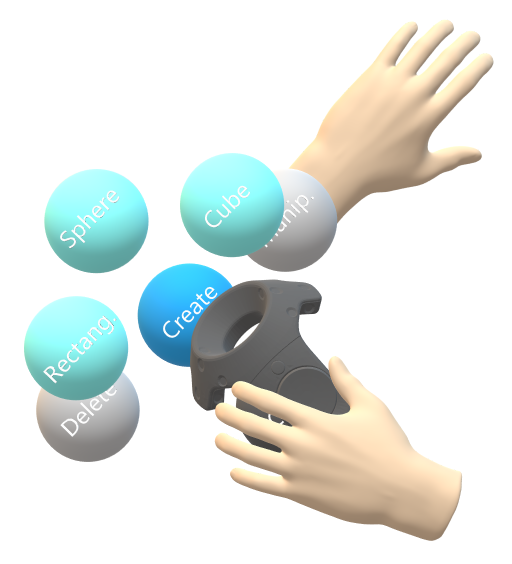
\includegraphics[scale=0.5]{Bilder/Hauptteil/konzept19a}
\centering
\caption{Interaktion und Erweiterung des \textit{3d button menu} nach~\cite[p.~36-37]{wheelpickerpiemenu}}
\label{fig:ballmodell}
\end{figure}

\subsubsection*{Kachel-Modell}
\noindent Das bekannte Kachel-Modell von Microsoft wurde ebenfalls in Betracht gezogen, zu sehen in Abbildung \ref{fig:kachelmodell}. Das Kachel-Modell besteht ausschließlich aus zweidimensionalen Rechtecken, und bietet wie das \textit{pie menu} oder das Kugel-Modell keine Tiefe. Vorteilhaft hierbei ist wiederum die simple Anordnung der Elemente. Die Kacheln werden über-, unter oder nebeneinander angeordnet und besitzen alle die gleichen Maße. Die Erweiterung des Kachel-Modells gestaltet sich in der hier beschriebenen Visualisierung schwierig, da ebenfalls wie beim Kugel-Modell eingeschlossene Elemente existieren, welche bei Erweiterung andere Elemente überdecken könnten.

\begin{figure}[h]
\captionsetup{width=.7\linewidth}
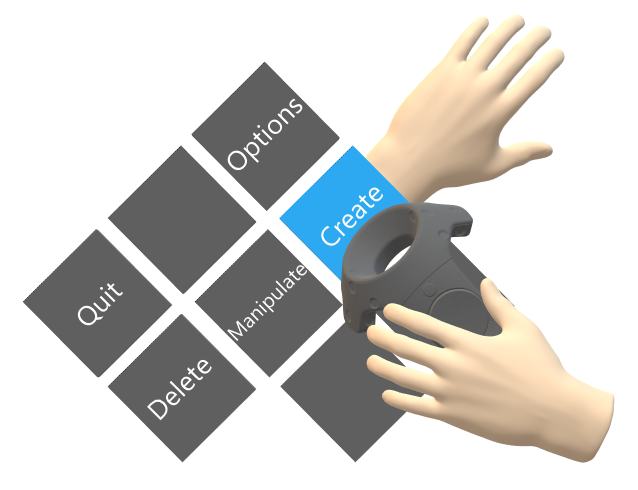
\includegraphics[scale=0.5]{Bilder/Hauptteil/konzept17}
\centering
\caption{Interaktion mit Kachel-Modell}
\label{fig:kachelmodell}
\end{figure}

\noindent Tabelle \ref{tab:interfacedesigns} listet die Merkmale und Eigenschaften der genannten Designs zusammengefasst auf.

\begin{table}[h]
\begin{center}
	\begin{tabular}{| l | p{10cm} |}
	\hline
	\multicolumn{1}{|c|}{\textbf{Designtyp}} & \multicolumn{1}{|c|}{\textbf{Eigenschaften und Merkmale}} \\ \hline
	\textit{3d wheel picker} & Deaktivierung nicht relevanter Funktionen durch Rotation, Tiefe und Rotation erschweren blinde Bedienung, Überdeckung durch Tiefe \\ \hline
	\textit{pie menu} & Keine Tiefe, Keine Rotation, Verdeckung, unterschiedliche Höhen und Breiten der Elemente \\ \hline
	\textit{3d button menu} & Einheitliche Elemente, Keine Tiefe,  Überdeckung, eingeschlossene Elemente, Überladung \\ \hline
	Kachel-Model & Keine Tiefe, einheitliche Elemente,  Eingeschlossene Elemente, Überdeckung \\ 
	\hline
	\end{tabular}
	\caption{Eigenschaften und Merkmale verwandter Interface-Designs}
	\label{tab:interfacedesigns}
\end{center}
\end{table}

\noindent Ein qualitativ hochwertiger Prototyp für ein Unterarm-Interface für VR, ist das vom YouTube-Kanal "CorvidDude" veröffentlichte Konzept, zu sehen in Abbildung \ref{fig:corviddude}. Das von CorvidDude entwickelte System, bietet Gestenerkennung, sowie ein an einen 3D \textit{Wheel picker} angelehntes Interface. Bei CorvidDude's Interface werden die UI-Elemente neben- und untereinander angebracht und können durch direkte Interaktion bedient werden~\citep{corviddude}.

\begin{figure}[h]
\captionsetup{width=.7\linewidth}
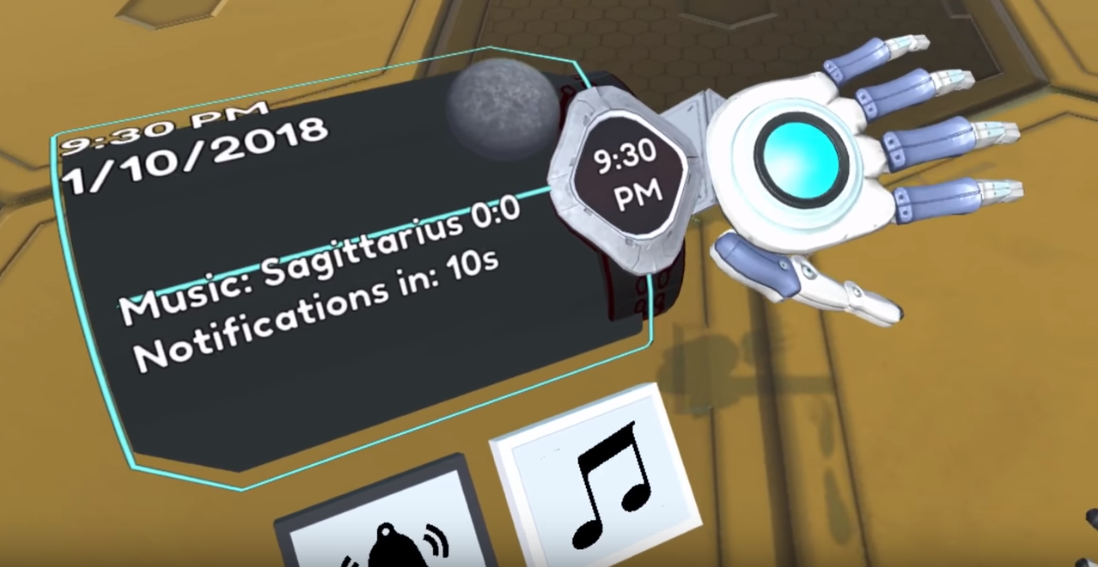
\includegraphics[scale=0.3]{Bilder/Hauptteil/arminterface}
\centering
\caption{Unterarm Prototyp für VR mit Gestenerkennung, vgl.~\citep{corviddude}}
\label{fig:corviddude}
\end{figure}

\subsubsection{Interfaceanforderungen}
Aus den vorangegangenen Richtlinien, Vorzügen der Positionierung und den Eigenschaften und Merkmale der verwandten Designs, entstanden die in Tabelle \ref{tab:interfaceanforderungen} aufgelisteten Anforderungen für die Gestaltung des prototypischen Interfaces. 
\begin{table}[h]
\begin{center}
  \begin{tabular}{| P{1cm} | p{12cm} |}
    \hline
     1. & \makecell[l]{Die Bedienung des Interfaces bezieht den  eigenen Körper mit ein}\\ \hline
     2. & \makecell[l]{Das Interface kommt ohne Scrollen oder  zusätzliche \\ Rotationsmechanismen aus}\\ \hline
     3. & \makecell[l]{Die Interface-Elemente sind zweidimensional und \\ einheitlich gestaltet}\\
    \hline
    4. & \makecell[l]{Es werden keine Elemente eingeschlossen die schwer \\ zu erweitern sind}\\
    \hline
    5. & \makecell[l]{Die Erweiterung einer Funktion überdeckt keine \\ anderen Funktionen}\\
    \hline
    6. & \makecell[l]{Es werden auffällige Farben für selektierte, aktivierte und \\ erweiterte Funktionen verwendet} \\
    \hline
    7. & \makecell[l]{Der Benutzer erhält unterstützendes Feedback wenn das Interface \\ blind bedient wird} \\ \hline
    8. & \makecell[l]{Funktionen, welche nicht zur Interaktion mit virtuellen Objekten \\ gedacht sind, unterscheiden sich in beliebiger Weise von den \\ interaktiven Funktionen}\\
    \hline
  \end{tabular}
  \caption{Interfaceanforderungen}
	\label{tab:interfaceanforderungen}
\end{center}
\end{table}

\subsubsection{Finales Interfacekonzept}
\noindent Der folgende Entwurf repräsentiert das finale Konzept für den zu entwickelnden Prototypen. Auf Grundlage der festgelegten Anforderungen und Richtlinien sowie des vorher beschriebenen Kachel-Modells und dessen Vorteile, entstand die Idee eines Designs, welches für weniger Überdeckung und Überladung sorgen soll. Dem in Abbildung \ref{fig:decisionmenu1} visualisierten Interface wird der Name \textit{decision menu} gegeben, da es einer Auswahl bekannt von Fragebögen oder Computer-Abfragen ähnelt, bei welchen die Auswahlmöglichkeiten unter- bzw.~nebeneinander platziert werden. Das \textit{decision menu} besteht wie das Kachel-Modell aus zweidimensionalen Bedienelementen, welche jedoch in der ersten Ebene nur nebeneinander angeordnet werden und somit Komplexität reduzieren.

\begin{figure}[h]
\captionsetup{width=.7\linewidth}
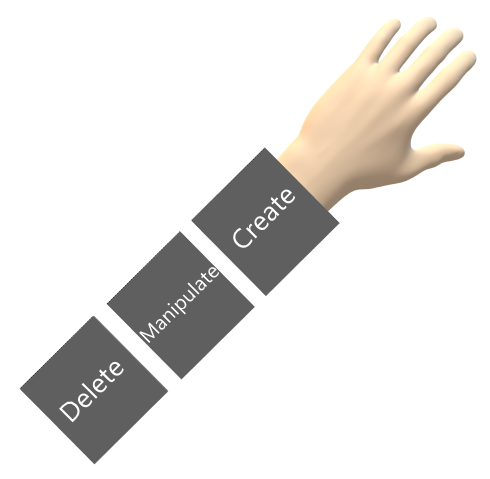
\includegraphics[scale=0.5]{Bilder/Hauptteil/konzept14}
\centering
\caption{Finales Konzept \textit{decision menu}}
\label{fig:decisionmenu1}
\end{figure}

\noindent Überdeckung findet aufgrund der horizontalen Ausrichtung der Elemente verringert statt. Die Erweiterung des \textit{decision menu} gestaltet sich leichter als bei den vorherigen Entwürfen, da es keine eingeschlossenen Elemente mehr gibt. Die Erweiterung der Funktionen wird durch Über- bzw.~Unterordnung der neuen Elemente gelöst. Dadurch werden keine anderen Funktionen überdeckt und bleiben auch bei Erweiterung einer Funktion komplett sichtbar. Die Bedienung wird beim \textit{decision menu} nicht nur durch die Kacheloptik, sondern auch durch die simple Positionierung derselbigen erleichtert. Eine blinde Bedienung ist somit einfacher als bei den vorherigen Modellen, da sowohl Überdeckung als auch Überladung geringer sind.

\begin{figure}[h]
\captionsetup{width=.7\linewidth}
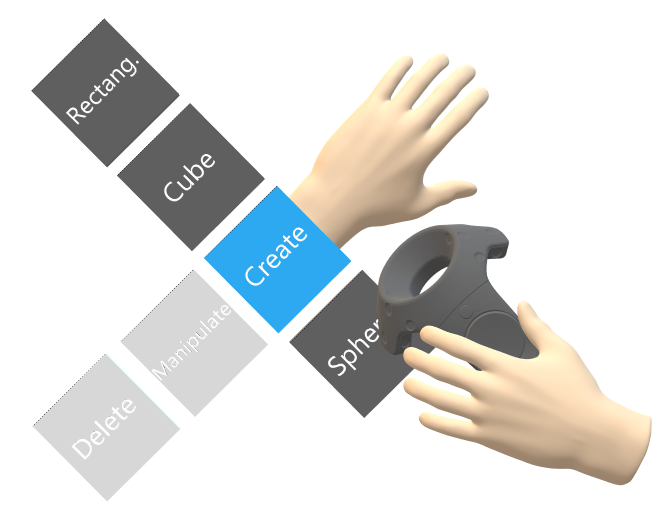
\includegraphics[scale=0.5]{Bilder/Hauptteil/konzept23}
\centering
\caption{Erweiterung des \textit{decision menu}}
\label{fig:decisionmenu2}
\end{figure}

\noindent Funktionen welche keine Auswirkungen auf die virtuell platzierten Objekte haben oder damit nicht in Zusammenhang stehen, werden an der Unterseite des Armes platziert. Dadurch wird die Oberseite entlastet und einer ungewollten Fehlauswahl vorgebeugt. 

\begin{figure}[h]
\captionsetup{width=.7\linewidth}
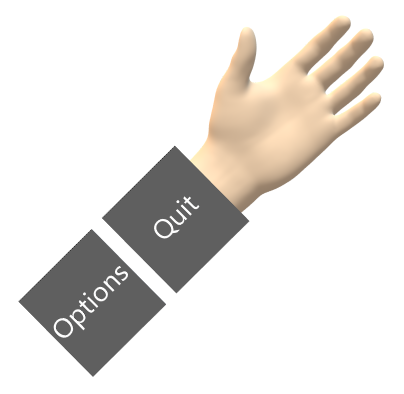
\includegraphics[scale=0.5]{Bilder/Hauptteil/konzept22}
\centering
\caption{Platzierung anwendungsspezifischer Funktionen}
\label{fig:decisionmenu3}
\end{figure}

\subsection{Implementation}
Dieses Kapitel beschreibt die Umsetzung des Prototypen und der dazugehörigen Anwendung. Zunächst werden die Tools und Frameworks erläutert, welche für die Implementation der Funktionen und Umgebung zu Hilfe genommen werden. Anschließend wird die praktische Realisierung in Textform zusammengefasst wiedergegeben. Dabei wird auf Probleme und besondere Ereignisse oder Hindernisse näher eingegangen.

\subsubsection{Verwendete Frameworks und Tools}
Zur Entwicklung der VR-Anwendung und des dazugehörigen körperbasierten Interfaces, werden diverse Programme verwendet, die sowohl VR-Unterstützung als auch nützliche Extras bieten. Unity vom Unternehmen \textit{Unity Technologies}, dient als Spiel-Engine und Entwicklungsumgebung. Verwendet wird dabei die Version 2018.3.11f1. Zum Schreiben des benötigten Codes wird Microsoft's Visual Studio Code verwendet. Für die Codeerkennung von Unity wird eine dementsprechende Erweiterung in Visual Studio Code integriert. Zur Benutzung des Vive Headsets sowie der Vive Controller und Vive Kameras, wird das Tool SteamVR~\citep{steamvr} in Unity importiert. SteamVR ist ausgestattet mit zahlreichen vordefinierten Funktionen und Möglichkeiten, mit VR-Hardware interagieren und VR-Anwendungen entwickeln zu können. Um das Gefühl für den eigenen Körper in VR zu erhöhen und damit die Qualität der Immersion zu verbessern, wird die Unity-Erweiterung FinalIK~\citep{finalik} verwendet. FinalIK nutzt u.a.~die Vive Hardware und erfasst die Beschaffenheit des Körpers des Trägers und kann dadurch eine vollständige virtuelle Kopie des Trägers und seiner Bewegungen im virtuellen Raum simulieren. Dadurch ist ein qualitativ hochwertiges Abbilden des Interfaces auf den Körper des Benutzers möglich.

\subsubsection{Umsetzung}
Die Umsetzung setzt sich zusammen aus Elementen, welche die Anwendung und dessen Gestaltung betreffen, als auch aus Elementen speziell für das Interface und die damit verbundenen Interaktionen. Zunächst wird die virtuelle Umgebung beschrieben, in welcher das Interface benutzt werden kann. Anschließend folgen Erläuterungen zur Implementation des Interfaces und der damit verbundenen Interaktion als auch Beschreibungen der Interface-Funktionen und der Benutzung der selbigen.\\

\noindent \textbf{Anwendung}\\
Die Anwendung ist schlicht und praktikabel gestaltet, da der Fokus dieser Arbeit auf dem Interface und der Verwendung dessen liegt. Die Umgebung besteht aus einem viereckigen Raum ohne Decke, dadurch soll sich der Benutzer nicht eingeengt fühlen und Platz nach oben für Manipulationen haben. Der Boden des Raumes wird mit einer Teleportations-Komponente versehen. Dadurch kann sich ein Benutzer bei Verwendung der entsprechenden Funktion, im Raum an beliebige Positionen und fest im Raum platzierte Teleportationspunkte teleportieren, um mit Objekten zu interagieren oder die Umgebung aus einem anderen Blickwinkel betrachten zu können. Jede Wand wird mit einer Kollidierungs-Komponente versehen. Somit kann der Benutzer nicht ungewollt aus dem Raum fallen. Der Boden und die Wände besitzen schlichte, unauffällige Texturen, sodass sich der Raum nicht ungewöhnlich oder fremd anfühlt. Auch alle erstellbaren Objekte besitzen Texturen. Die Texturen der primitiven Körper bestehen jedoch ausschließlich aus einfachen Farben wie rot, grün oder blau. Die Texturen der Objekte werden bewusst in den RGB-Farben gehalten, um die Objekte unterscheiden zu können und die Objekte für jeden subjektiven Kontext passend zu machen. Das Modell des Benutzers ist eine von FinalIK mitgelieferte Vorlage, welche an einen Crashtest-Dummy angelehnt ist. Das Modell nimmt dadurch keine geschlechterspezifische Rolle an, was für eine positive Benutzererfahrung bei allen Geschlechtern sorgen soll. Das Modell wird mit einer hautähnlichen Farbe versehen, um ein natürlicheres Gefühl bei der Verwendung und Interaktion mit dem Modell herzustellen.\\

\noindent \textbf{Interface}\\
Das Interface wird am nicht dominanten Arm des Dummy-Modells angebracht. Durch das FinalIK-Plugin können dem Dummy-Modell sogenannte \textit{Bones} und Kalibrierungs-Komponenten zugeordnet werden. Somit kann das Dummy-Modell an den Körper eines Benutzers angepasst werden, um für eine größere Immersion und genauere Eingaben sowie Bewegungen zu sorgen. Der Arm teilt sich somit in mehrere \textit{Bones} auf, welche bei der Positionierung und Fixierung des Interfaces hilfreich sind. Das Interface selbst besteht aus einem \textit{Canvas}, welches im \textit{WorldSpace} platziert wurde. Durch die \textit{WorldSpace} Einstellung, wird die Anbringung am Arm des Benutzers erst möglich, da ein im \textit{ScreenSpace} platziertes Interface direkt vor einer Kamera platziert wird und im dreidimensionalen Raum nicht frei beweglich ist, was für diese Arbeit jedoch wichtig ist. Die Rotation und Translation des Interfaces wird hauptsächlich durch das Modell und die zugeordneten \textit{Bones} sowie ein Rotationsskript von FinalIK geregelt. Da das Interface jedoch bei ausschließlicher Verwendung der FinalIK-Komponenten noch nicht am Arm fixiert ist und sich mit dem Arm auch noch nicht mitdreht, wird ein zusätzliches selbstgeschriebenes Skript eingebaut, welches das Interface am Arm fixiert und abhängig von der Hand-Rotation mitdreht. Auf der ersten Ebene, welche sich auf der oberen Seite des Unterarms befindet, werden die objektspezifischen Funktionen angebracht. Darunter die Funktionen zur Manipulation und Erstellung von Objekten, in der Anwendung \textit{Manipulate} und \textit{Create} genannt. Die englische Sprache wird für alle Interaktionen, Hinweise und Bezeichnungen verwendet, um die Anwendung international einsetzbar zu machen. Die objektspezifischen Funktionen der ersten Ebene werden nebeneinander angebracht und erstrecken sich somit auf der horizontalen Achse des Armes des Dummy-Modells. Die zweite Ebene der objektspezifischen Funktionen, erstreckt sich auf der vertikalen Achse des Armes. Das bedeutet, dass erweiterte Funktionen über- oder unter den Funktionen der ersten Ebene angebracht sind, ohne die erste Ebene zu verdecken. Zur Erweiterung der Manipulationsfunktion gehören die Standard-Manipulationen \textit{Translate}, \textit{Rotate} und \textit{Scale}, auf welche später in diesem Kapitel eingegangen wird. Die Erweiterung der \textit{Create}-Funktion umfasst die drei primitiven Körper Würfel, Kugel und Zylinder. Anwendungsspezifische Funktionen bzw.~Funktionen ohne weitere Kategorisierung, werden auf der unteren Seite des Unterarms des Dummy-Modells angebracht. Dadurch soll der Fokus der Interaktion auf die Objekte verstärkt werden und die Komplexität und Bedienung des Interfaces verringert und erleichtert werden. Zu den nicht kategorisierten bzw.~anwendungsspezifischen Funktionen gehört das Löschen von Objekten, in der Anwendung \textit{Delete} genannt, und das Beenden der Anwendung, in der Anwendung mit \textit{Quit} tituliert. Die Quit-Funktion befindet sich bewusst weiter hinten am Unterarm, um die Wahrscheinlichkeit eines versehentlichen Schließens der Anwendung zu verringern. Zusätzliche oder neue Funktionen können beliebig auf den Achsen auf der Ober- oder Unterseite des Armes platziert werden, wenn die Ebenen und deren Bedeutung berücksichtigt wird. Die erste Ebene symbolisiert Obermenüs, wohingegen die zweite Ebene Untermenüs bzw.~Funktionen ohne weitere Unterkategorien darstellt. Aufgeklappte, aktive und markierte Funktionen werden farblich hervorgehoben, um ein visuelles Feedback bei der Bedienung des Interfaces zurückzugeben. Nach Vos reagieren Menschen besonders auf gelbe oder grüne sowie auf helle Farben~\citep{colors}. Daraus resultieren die vergebenen Farben für die verschiedenen visuellen Feedbacks bei der Verwendung des Interfaces, zu sehen in Abbildung \ref{fig:interfaceimp}. Aufgeklappte Funktionen werden demnach türkis dargestellt, aktivierte Funktionen gelb und markierte Funktionen hellblau. Die Standardfarbe für alle Funktionen ist weiß.

\begin{figure}[h]
\captionsetup{width=.7\linewidth}
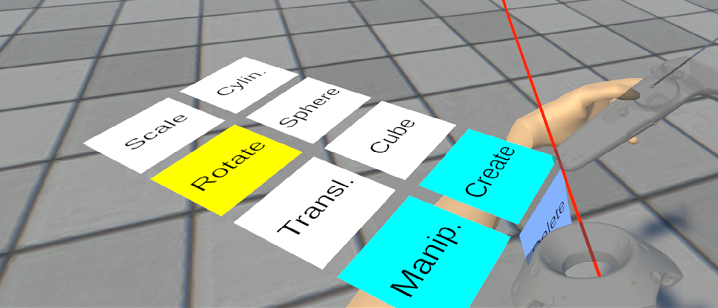
\includegraphics[scale=0.6]{Bilder/Hauptteil/Bearbeitet/Interface}
\centering
\caption{Interfaceimplementation}
\label{fig:interfaceimp}
\end{figure}

%\noindent \textbf{Interfaceinteraktion}\\

\noindent \textbf{Funktionen}\\
In diesem Abschnitt werden die Interface- und Anwendungsfunktionen und deren Benutzung näher erläutert. Dabei wird der Zweck jeder Funktion beschrieben und die Verwendung und Auswirkung verdeutlicht. Um die Bedienung der Controller besser zu verstehen dient Abbildung \ref{fig:vivecontrollerextended}, welche die verschiedenen Buttons visualisiert.

\begin{figure}[h]
\captionsetup{width=.7\linewidth}
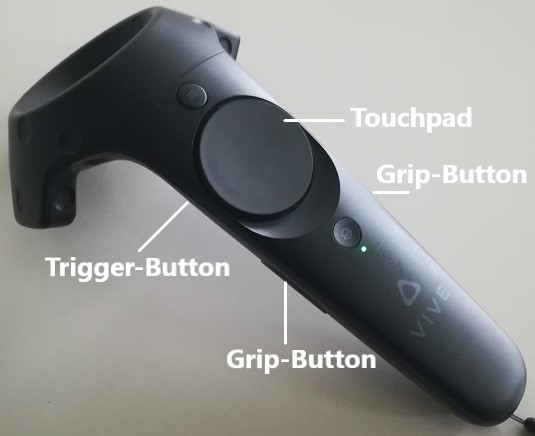
\includegraphics[scale=0.5]{Bilder/Hauptteil/vivecontrollerextended}
\centering
\caption{Vive Controller mit Bezeichner}
\label{fig:vivecontrollerextended}
\end{figure}

\noindent Die Teleportation des Benutzers wird durch eine Touchpad-Funktion ermöglicht. Dazu wird das Touchpad des rechten Controllers gedrückt und gehalten, und anschließend ein beliebiger Punkt im Raum anvisiert. Die Teleportation wird durch eine gestrichelte Kurve und einen Auftreffpunkt repräsentiert, wie in Abbildung \ref{fig:teleportation} zu sehen. Nach Loslassen des Touchpad-Buttons wird der Benutzer zum ausgewählten Ort teleportiert.

\begin{figure}[h]
\captionsetup{width=.7\linewidth}
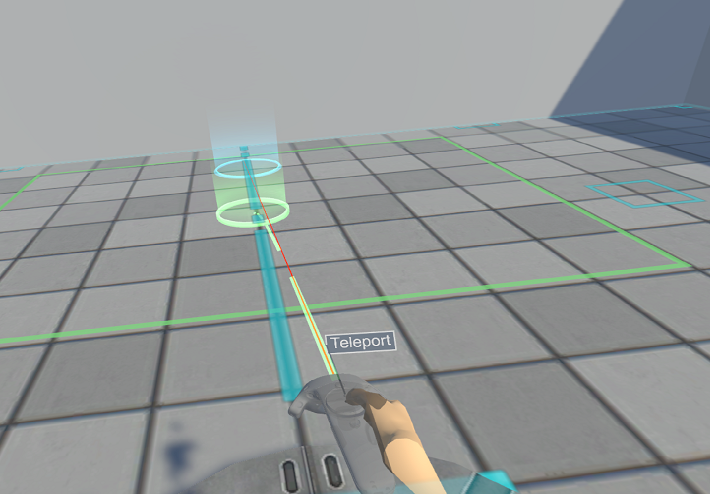
\includegraphics[scale=0.5]{Bilder/Hauptteil/Bearbeitet/Teleport}
\centering
\caption{Teleportationsfunktion}
\label{fig:teleportation}
\end{figure}

\noindent Objekte werden durch das Markieren eines Körper-Buttons und anschließendes Drücken des Trigger-Buttons des rechten Controllers erstellt und in der Mitte des Raumes platziert.\\
Um ein Objekt zu (de-)selektieren, wird eine Laserpointer-Technik verwendet. Dadurch kann auch mit weiter entfernten Objekten gearbeitet werden, ohne in deren unmittelbarer Nähe sein zu müssen. Der Laserpointer wird am rechten Controller angebracht und besitzt zwei Farben, welche den aktuellen Status des Laserpointers darstellen. Die Nichtverwendung wird durch einen roten, die Aktivierung durch einen blauen Strahl repräsentiert. Wird der Trigger-Button des rechten Controllers gedrückt, während ein selektierbares Objekt anvisiert wird, so wird das Objekt ausgewählt und gelb eingefärbt, um die Selektion, visualisiert in Abbildung \ref{fig:selektion}, zu bestätigen. Die Deselektion wird durch erneutes Drücken des Trigger-Buttons durchgeführt.

\begin{figure}[h]
\captionsetup{width=.7\linewidth}
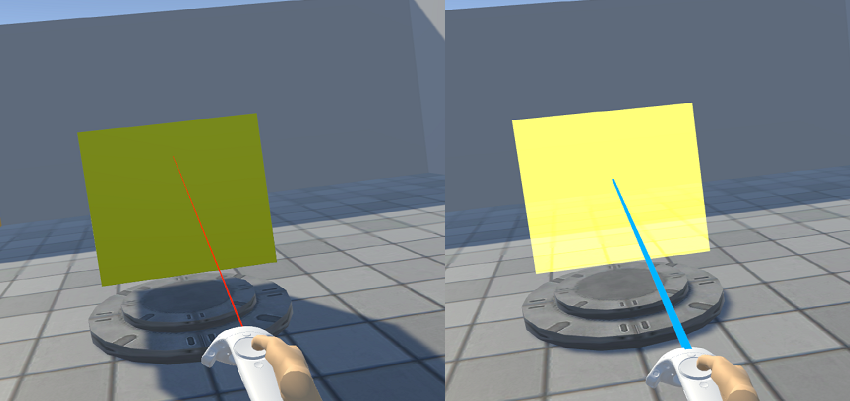
\includegraphics[scale=0.5]{Bilder/Hauptteil/Bearbeitet/SelektionMerge}
\centering
\caption{Markieren und Selektieren eines Würfels}
\label{fig:selektion}
\end{figure}

\noindent Die Translation von selektierten Objekten, zu sehen in Abbildung \ref{fig:translation}, setzt die Aktivierung der Translations-Funktion voraus. Ist die Funktion aktiviert, so kann ein Objekt durch das Drücken und Halten des linken Grip-Buttons frei im Raum bewegt werden. Wird der Grip-Button losgelassen so verweilt das Objekt an der zuletzt erreichten Position.

\begin{figure}[h]
\captionsetup{width=.7\linewidth}
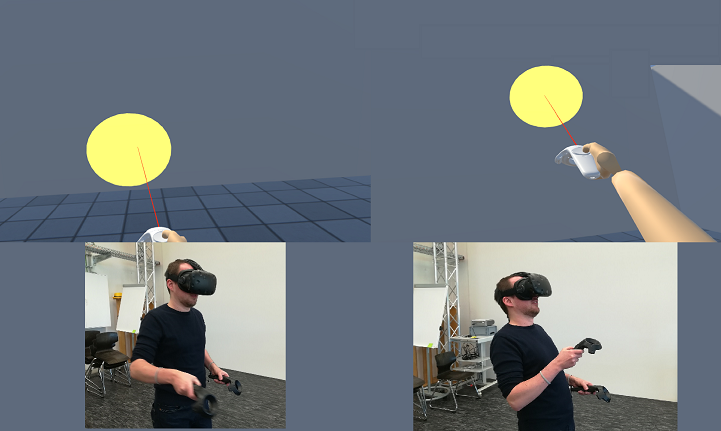
\includegraphics[scale=0.6]{Bilder/Hauptteil/Bearbeitet/TranslationMerge}
\centering
\caption{Verwendung der Translationsfunktion}
\label{fig:translation}
\end{figure}

\noindent Eine Rotation setzt ebenfalls eine Aktivierung der Funktion voraus, als auch ein selektiertes Objekt. Sind beide Voraussetzungen gegeben, kann ein Objekt wie in Abbildung \ref{fig:rotation} durch Drücken und Halten des linken Grip-Buttons am rechten Controller sowie eine beliebige Rotationsrichtung rotiert werden.

\begin{figure}[h]
\captionsetup{width=.7\linewidth}
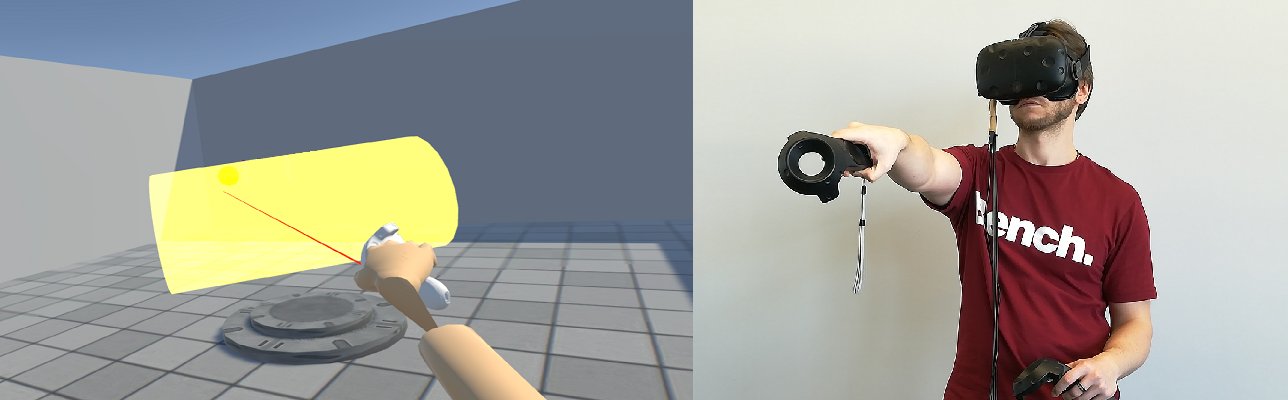
\includegraphics[scale=0.35]{Bilder/Hauptteil/Bearbeitet/RotationMerge}
\centering
\caption{Rotieren eines Objektes}
\label{fig:rotation}
\end{figure}

\noindent Die Skalierung ist in dieser Arbeit die einzige Funktion, die eine zweihändige Geste voraussetzt. Nach Aktivierung der Funktion und Auswählen eines Objektes kann ein Objekt skaliert werden, indem der rechte Grip-Button des linken und der linke Grip-Button des rechten Controllers gedrückt und gehalten werden, und die Controller voneinander weg oder zueinander hin bewegt werden. Die Skalierungs-Geste entspricht der Vergrößern-Verkleinern-Geste, bekannt aus der Verwendung eines Smartphones. Abbildung \ref{fig:skalierung} verdeutlicht die Funktionsweise.

\begin{figure}[h]
\captionsetup{width=.7\linewidth}
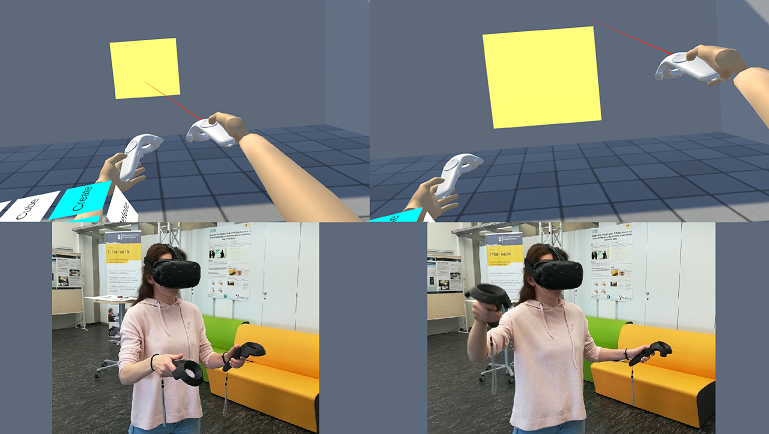
\includegraphics[scale=0.6]{Bilder/Hauptteil/Bearbeitet/SkalierungMerge}
\centering
\caption{Verwendung der Skalierungsfunktion}
\label{fig:skalierung}
\end{figure}

\noindent Das Löschen von Objekten, setzt ein ausgewähltes Objekt voraus. Eine Markierung und anschließende Aktivierung durch den Trigger-Button des rechten Controllers löscht das ausgewählte Objekt und hebt die Auswahl auf.\\
\\
Der Benutzer hat die Möglichkeit die Anwendung jederzeit zu beenden. Dazu wird der Quit-Button markiert und mit Drücken des Trigger-Buttons des rechten Controllers bestätigt. Der Benutzer gelangt daraufhin ins SteamVR-Hauptmenü zurück.\\
\\
Um das Interface blind bedienen zu können, wird eine Technik verwendet, welche den aktuellen Sichtbereich des Benutzers speichert und überprüft, ob eine Funktion momentan markiert, aber nicht zu sehen ist. Ist eine Funktion markiert aber nicht sichtbar, so wird der Titel des markierten Buttons wie in Abbildung \ref{fig:blind} vor der virtuellen Kamera angezeigt.

\begin{figure}[h]
\captionsetup{width=.7\linewidth}
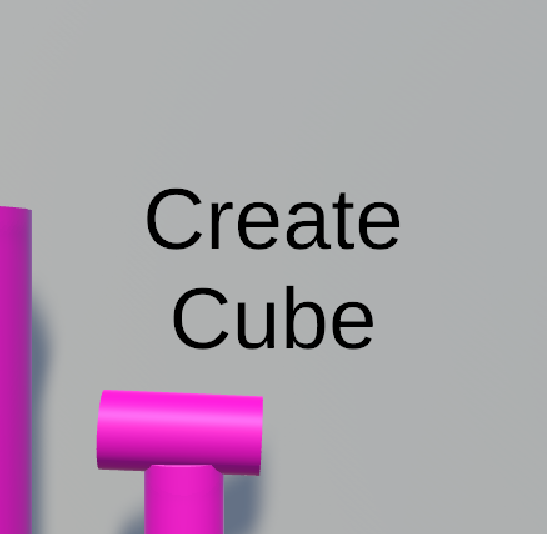
\includegraphics[scale=0.5]{Bilder/Hauptteil/Bearbeitet/Blind}
\centering
\caption{Einblendung eines Funktionstitels bei blinder Bedienung}
\label{fig:blind}
\end{figure}

\subsubsection{Probleme und Hindernisse}
Bei der Entwicklung und Implementation des Interfaces als auch der damit verbundenen Funktionen, kommt es regelmäßig zu Verzögerungen.  Aufgrund der unterschiedlichen Komplexität dauern Lösungen unterschiedlich lange und nehmen dadurch einen wesentlichen Teil bei der Entwicklung ein. Problematisch ist der Umgang mit den Erweiterungen. Da SteamVR und FinalIK von unterschiedlichen Herstellern entwickelt werden, kommt es teilweise zu Interferenzen bei der Implementation, woraufhin Lösungen gefunden werden müssen, um beide Erweiterungen ohne Fehler verwenden zu können. Um die Interferenzen aufzulösen, werden Funktionsabschnitte gebildet. Das bedeutet, dass z.B.~die Translations-Funktion zu sehen in Abbildung \ref{fig:translation}, ausschließlich Skripte und Komponenten des SteamVR-Plugins verwendet. Das Dummy-Modell hingegen verwendet nur Skripte des FinalIK-Plugins. Dadurch wird vermieden, dass sich Skripte in der Verarbeitung von Informationen oder Kommunikation stören. Auch die Rotation von Objekten gestaltet sich als schwierig, da eine Lösung implementiert werden soll, welche abhängig von der aktuellen Position des Benutzers zu jeder Zeit die gleichen Aktionen ausführt. Das bedeutet, dass die unterschiedlichen Achsen von Objekt und Benutzer gespiegelt und passend übersetzt werden müssen, je nachdem in welchem Winkel der Benutzer zum Objekt steht, da nur somit eine stetig übereinstimmende visuelle Repräsentation der Rotation möglich ist. Ein weiteres Hindernis ist die Platzierung auf und die Rotation des Interfaces mit dem Arm des Dummy-Modells, da sich der Arm standardmäßig nicht mit der Hand mit rotiert. Dadurch müssen zusätzliche Skripte entwickelt und weitere mitgelieferte Komponenten eingebunden und konfiguriert werden. Ein kleines, jedoch wichtiges Feature, welches mehrmals angepasst werden muss, ist die Interaktion der Bedienelemente. Die Buttons des Interfaces direkt mit dem Controller bedienen zu können, darunter das Aufklappen und Aktivieren von Funktionen, stellt sich als schwierig heraus, wird jedoch mit ansteigendem Wissen und Kreativität zunehmend einfacher und schließlich gelöst. Kleinere Probleme wie Fehlkonfigurationen, Versuch und Irrtum Ansätze oder Ausfälle der Hardware erschweren und verzögern die Implementation zusätzlich, jedoch nicht gravierend.

\subsection{Evaluation}
In diesem Abschnitt wird näher auf die Evaluation des entwickelten Systems, bestehend aus Anwendung und Interface, eingegangen. Dabei wird u.a.~erläutert mit welcher Methode evaluiert wird, wie die dabei verwendeten Räumlichkeiten und Variablen aussehen, wie das System bewertet wird und wie die Ergebnisse und deren Interpretation ausgefallen sind.

\subsubsection{Aufbau}
Die Evaluation des Systems wird nach dem DECIDE-Framework von~\citep{decidebook} konzipiert und durchgeführt. DECIDE steht dabei für \textit{\textbf{D}etermine the goals}, \textit{\textbf{E}xplore the questions}, \textit{\textbf{C}hoose the evaluation methods}, \textit{\textbf{I}dentify the practical issues}, \textit{\textbf{D}ecide how to deal with the ethical issues}, \textit{\textbf{E}valuate, analyze, interpret, and present the data}. Das Ziel der Evaluation ist, die Usability und Bedienung des Systems zu überprüfen. Usability wird in dieser Arbeit nach der ISO Norm 9241 betrachtet und untersucht. Dabei wird unter Usability die Effektivität, Effizienz und Zufriedenheit eines Benutzers bei der Erreichung von bestimmten Zielen in speziellen Umgebungen verstanden~\citep{usability}. Zur Untersuchung der Usability wird der \textit{System Usability Scale} (SUS) von J. Brooke~\citep[p.~189-196]{sus} als Grundlage für die Befragung der Testpersonen verwendet. Der SUS beinhaltet die folgenden zehn Fragen, aufgelistet in Tabelle \ref{tab:susfragen}, welche das System und dessen Usability durch Werte von 1 für "Stimme überhaupt nicht zu" bis 5 für "Stimme voll und ganz zu" bewertbar und überprüfbar macht.

\begin{table}[h]
\begin{center}
  \begin{tabular}{| P{1cm} | p{12cm} |}
    \hline
     1. & \makecell[l]{I think that I would like to use this system frequently}\\ \hline
     2. & \makecell[l]{I found the system unnecessarily complex}\\ \hline
     3. & \makecell[l]{I thought the system was easy to use}\\ \hline
    4. & \makecell[l]{I think that I would need the support of a technical person\\ to be able to use this system}\\
    \hline
    5. & \makecell[l]{I found the various functions in this system were well integrated}\\
    \hline
    6. & \makecell[l]{I thought there was too much inconsistency in this system} \\
    \hline
    7. & \makecell[l]{I would imagine that most people would learn to use\\ this system very quickly}\\
    \hline
    8. & \makecell[l]{I found the system very cumbersome to use}\\
    \hline
    9. & \makecell[l]{I felt very confident using the system}\\
    \hline
    10. & \makecell[l]{I needed to learn a lot of things before I could\\get going with this system}\\
    \hline
  \end{tabular}
  \caption{System Usability Scale Fragen nach Reihenfolge sortiert}
	\label{tab:susfragen}
\end{center}
\end{table}

\noindent Zusätzlich zum SUS wird die Umfrage durch Fragen nach der bisherigen Erfahrung mit VR und HMDs sowie dem Alter und dem Geschlecht erweitert. Die Beschreibung der VR-Erfahrung erstreckt sich von "Ich habe noch nie von VR und HMDs gehört" über "Ich habe schon einmal mit VR und HMDs gearbeitet oder gespielt" bis hin zu "Ich verwende VR Hardware regelmäßig und kenne mich gut aus". Die Räumlichkeit in der die Evaluationsdurchführung stattfindet, wird mithilfe des SteamVR-Plugins auf circa 4.0 x 3.0 Meter gemessen. Die gemessene Größe und damit die Limitierung der Bewegungsfreiheit, wird dem Träger der HTC Vive bei der Durchführung durch rote Linien auf dem Bildschirm angezeigt. Der Raum bietet helle Deckenleuchten und ist somit unabhängig von äußeren Umweltgegebenheiten verwendbar. Ebenfalls wird der virtuelle Raum, zu sehen in Abbildung \ref{fig:evaraum}, für die Evaluation angepasst.

\begin{figure}[h]
\captionsetup{width=.7\linewidth}
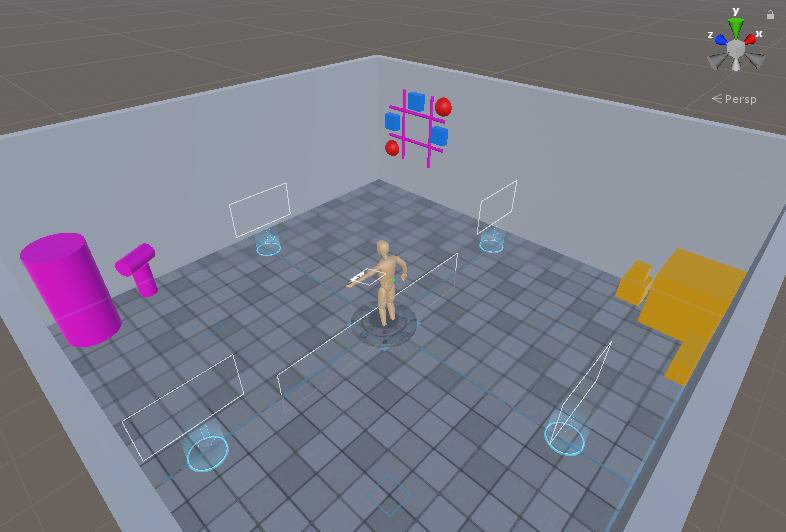
\includegraphics[scale=0.5]{Bilder/Hauptteil/BildRaum}
\centering
\caption{Angepasster virtueller Raum für Evaluation}
\label{fig:evaraum}
\end{figure}

\noindent Die Testumgebung wird mit Objekten gefüllt, welche sowohl als Orientierungshilfe zur Erfüllung der gestellten Aufgaben, als auch als Interaktionsmöglichkeit dienen. Zu den Aufgaben gehört das Teleportieren, Erstellen von Objekten, Selektieren und Deselektieren von Objekten, die Translation, Rotation und Skalierung von Objekten, sowie das Löschen von Objekten, die blinde Bedienung und das Beenden der Anwendung. Die Aufgaben sind unterschiedlich schwer und sollen den Fortschritt beim Erlernen der Bedienung des Interfaces, als auch den Funktionsumfang dessen darstellen. Wird einem Benutzer beim Testen schlecht oder äußert ein Tester den Wunsch die Anwendung und den Test zu beenden, so ist dem Tester die Ausrüstung unverzüglich abzunehmen und die Anwendung zu beenden. Das Recht des Testers auf die Umfrage verwirkt damit jedoch nicht. Der Test und die Umfrage wurden in einer Pilotstudie mit zwei Personen im Alter von 22 bzw.~36 Jahren getestet. Dabei hat sich ergeben, dass Aufgaben teilweise noch zu ungenau beschrieben sind und die Kalibrierung nochmals überarbeitet werden muss, da die aktuell implementierte Kalibrierung beim Benutzen von Funktionen zurückgesetzt wird und die Testpersonen die UI-Elemente somit nicht mehr bedienen können.

\subsubsection{Durchführung}
Die Evaluation wurde in einem lichtdurchfluteten Raum mit Raumtemperatur durchgeführt. Männer und Frauen wurden in beliebiger Reihenfolge nacheinander über einen Testzeitraum von acht Stunden hinweg getestet. Dafür musste jeder Proband vorab eine Einverständniserklärung unterzeichnen und bekam daraufhin ein Einleitungsvideo zu sehen, welches auf die anschließenden Aufgaben vorbereitete und die Verwendung des Interfaces darstellte. Jeder Testperson wurde in gleichem Maße bei der Verwendung der Ausrüstung und der Einnahme der Startposition geholfen. Zu Anfang jedes Testdurchlaufes wurde die Testperson über ein Kalibrierungs-Skript und zwei Tastendrücke kalibriert, um das Dummy-Modell auf die tatsächliche Größe des Testers oder der Testerin anzupassen, und somit die Bedienung des Interfaces zu erleichtern. Für jede Testperson wurde die Zeit für die Erfüllung aller Aufgaben gestoppt. Die Höchstdauer für die Erfüllung aller Aufgaben betrug 20 Minuten. Jeder Testperson wurden die gleichen Aufgabestellungen gegeben, Hilfestellungen wenn nötig geboten, und Hinweise aufgesagt. Die Aufgaben wurden nach Schwierigkeit angeordnet und wurden wenn gewünscht wiederholt. Nach einem Testdurchlauf wurde die jeweilige Testperson gebeten die Umfrage auszufüllen und damit den Test abzuschließen. Probleme wie das Ausfallen der Hardware oder die Falschkalibrierung der Testperson, wurde über den Neustart der Anwendung und dem erneuten Einnehmen der Startposition gelöst. Traten Probleme inmitten des Testes auf, so wurde die Anwendung neu gestartet, und die zuletzt aktive Aufgabe wiederholt.

\subsubsection{Ergebnisse}
Getestet wurden insgesamt 22 Personen zwischen 19 und 32 Jahren mit Informatik-Affinität. Die 22 Testpersonen bestehen aus 13 Männern und 9 Frauen. Die durchschnittliche Durchführungszeit aller Personen beläuft sich auf 7 Minuten. Im Durchschnitt haben die Männer 6 Minuten und 45 Sekunden, die Frauen 8 Minuten und 12 Sekunden für alle Aufgaben benötigt. Die erhaltenen Werte der Testpersonen werden nach dem SUS-Bewertungsmodell von J.~Brooke berechnet. Dabei werden die Antwortwerte jeweils um 1 verringert, sodass die Werte von 0 bis 4 reichen. Eine 0 steht bei einer positiven Aussage wie "Ich fand die Funktionen des Systems gut integriert" für "Stimme überhaupt nicht zu", eine 4 für "Stimme voll und ganz zu". Bei einer negativen Aussage wie "Ich fand das System unnötig komplex" verhalten sich die Werte umgekehrt. Eine 0 entspricht vollster Zustimmung, eine 4 steht für keine Zustimmung. Die erhaltenen Werte jeder Testperson werden zusammengezählt und mit 2.5 multipliziert. Der daraus resultierende Wert entspricht dem erzielten SUS-Score, welcher von 0 bis 100 reicht. 100 Punkte entsprechen demnach einer perfekten Usability, 0 Punkte hingegen einer miserablen Usability~\citep[p.~189-196]{sus}. Die Auszählung aller Testpersonen ergibt einen SUS-Score des Systems von 1765 von 2200 möglichen Punkten. Die erreichten Punkte ergeben umgerechnet in Prozent einen Wert von 80,23\%. Die erzielten 80,23\% ergeben für die Usability nach dem SUS-Bewertungsmodell zu sehen in Abbildung \ref{fig:sus} die Note B bis A, was einer guten bis exzellenten Usability entspricht. Dem entwickelten System kann demnach eine Eignung für junge Erwachsene für die Modellierung von 3D-Objekten in VR bei Verwendung eines körperbasierten Interfaces zugeschrieben werden.

\begin{figure}[h]
\captionsetup{width=.7\linewidth}
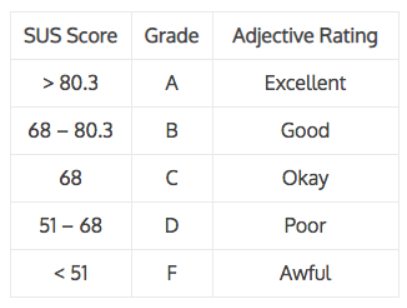
\includegraphics[scale=0.75]{Bilder/Hauptteil/susscore}
\centering
\caption{SUS-Score Interpretation nach~\citep{susscore}}
\label{fig:sus}
\end{figure}

\noindent Der Männeranteil hat die Usability des Systems umgerechnet in Prozent mit 82,12\%, der Frauenanteil mit 77,5\% eingeschätzt. Die Differenz von Männern und Frauen beträgt demnach 4,62\%. Der Männeranteil hat das System somit besser eingeschätzt, als der Frauenanteil. Der niedrigste errechnete SUS-Score entspricht 47,5, der höchste Wert 100 Punkten. In Abbildung \ref{fig:susscorealler} sind die erreichten SUS-Scores von Männern und Frauen aufgeführt, zusammen mit dem Durchschnitt und der Standardabweichung jeder Erfahrungsstufe.

\begin{figure}[h]
\captionsetup{width=.7\linewidth}
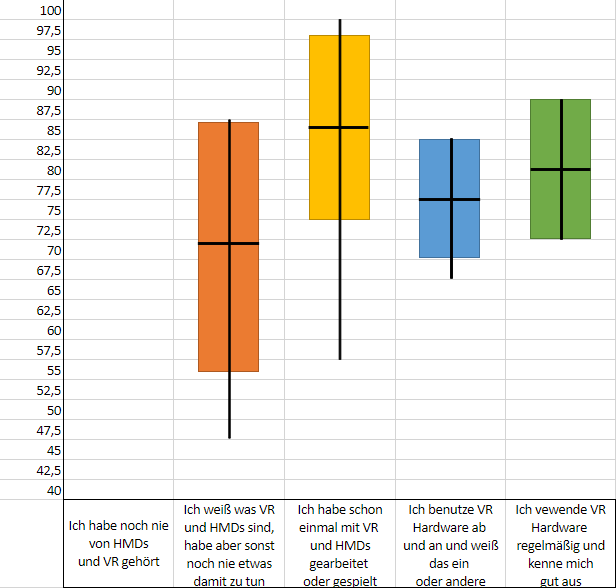
\includegraphics[scale=0.8]{Bilder/Hauptteil/susvrstandardabweichung}
\centering
\caption{SUS-Score Verteilung in Abhängigkeit zur VR-Erfahrung}
\label{fig:susscorealler}
\end{figure}

\noindent Die Erfahrung von Männern und Frauen, abgebildet in Schaubild \ref{fig:vrerfahrung}, verteilt sich auf die Werte 1 bis 4, bzw.~1 bis 3.

\begin{figure}[h]
\captionsetup{width=.7\linewidth}
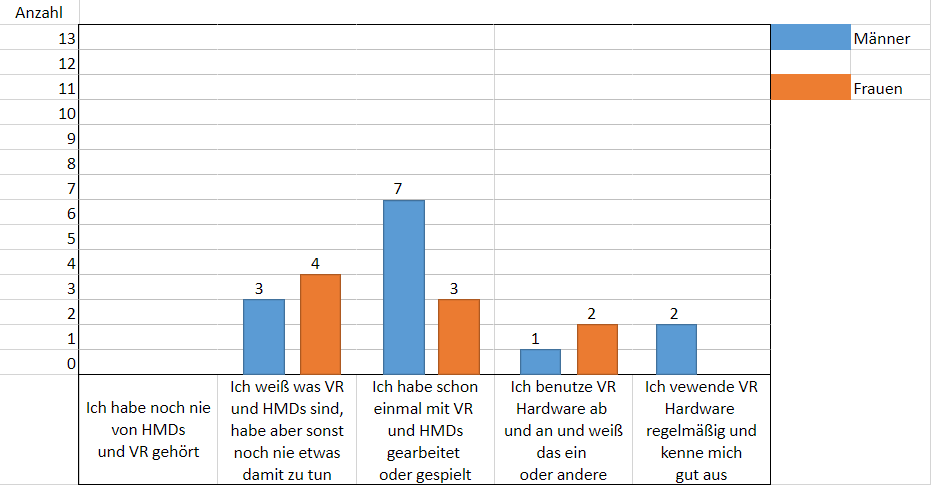
\includegraphics[scale=0.6]{Bilder/Hauptteil/vrerfahrungalle}
\centering
\caption{VR-Erfahrung aller Testpersonen}
\label{fig:vrerfahrung}
\end{figure}

\noindent Die Frage mit den meisten 4-er Wertungen ist Frage 2, welche eine positive Aussage ist, mit 14 4-er Wertungen. Die am negativsten bewerteten Fragen sind Frage 4, 6 und 10. Die Verteilung in Abbildung \ref{fig:negativstefragen} zeigt die Anzahl der vergebenen Negativwerte der jeweiligen Frage.

\begin{figure}[h]
\captionsetup{width=.7\linewidth}
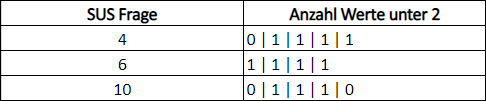
\includegraphics[scale=0.8]{Bilder/Hauptteil/negativsteFragen}
\centering
\caption{Am negativsten bewertete Fragen des SUS}
\label{fig:negativstefragen}
\end{figure}

\noindent Die größte Differenz zwischen Männern und Frauen, besteht bei Frage 4 und 7. Dabei ist eine Differenz zu messen von 5,4\% bzw.~10,10\%. Die am höchsten bewertete Frage der Männer ist Frage 9 mit 46 von 52 möglichen Punkten, die am höchsten bewerteten Fragen der Frauen sind Frage 3 und 7 mit jeweils 32 von 36 Punkten. Abbildung \ref{fig:fragensusscores} zeigt das erreichte Maximum und Minimum, sowie Durchschnitt und Standardabweichung jedweder SUS-Frage. Dabei entspricht die Zahl 4 einer vollen Zustimmung, die Zahl 1 einer totalen Ablehnung nach dem SUS-Bewertungsmodell.

\begin{figure}[h]
\captionsetup{width=.7\linewidth}
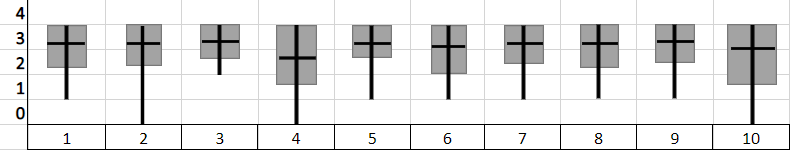
\includegraphics[scale=0.75]{Bilder/Hauptteil/susfragenstandardabweichung}
\centering
\caption{Bewertungen der SUS-Fragen}
\label{fig:fragensusscores}
\end{figure}

\noindent Abbildung \ref{fig:fragensusscores} verdeutlicht auch, dass für jede Frage Top-Bewertungen von 4 Punkten erreicht wurden, wohingegen für nur drei Fragen Werte von 0 vergeben wurden. Die durchschnittliche Durchführungszeit pro Erfahrungsstufe ist in Abbildung  visualisiert. Danach gibt es eine Differenz von einer bis knapp drei Minuten zwischen den erfahrensten und den weniger erfahrenen Testpersonen. Eine kontinuierliche Verkürzung der Durchführungszeit abhängig von der VR-Erfahrung kann damit ausgeschlossen werden.
 
\begin{figure}[h]
\captionsetup{width=.7\linewidth}
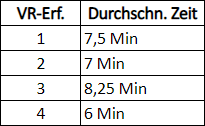
\includegraphics[scale=1.0]{Bilder/Hauptteil/durchschnittzeitvrerf}
\centering
\caption{Durchschn.~Durchführungszeit aller Erfahrungsstufen}
\label{fig:durchschnittzeitalle}
\end{figure}

\noindent Verglichen mit dem auf Gestenerkennung und -Steuerung basierenden System für 3D-Modellierung in VR von Alkemade et al., wobei 11 Personen zwischen 22 und 31 Jahren ebenfalls mit der SUS-Studie getestet wurden, erreicht das in dieser Arbeit entwickelte System einen geschätzt 20\% höheren SUS-Score. Gemeinsam mit dem System von Alkemade et al.~hat das entwickelte System dieser Arbeit die signifikante Differenz von Frage 4 zwischen den männlichen und weiblichen Testpersonen~\citep{alkemade}. Demnach bräuchten die weiblichen Testpersonen von Alkemade et al.'s System, ebenfalls eher technische Unterstützung bei der Verwendung des Systems, als die getesteten Männer.
\\
\\
Auf mündliche Nachfrage zur Usability des Systems, gaben fünf von 22 Personen an, dass die Selektion von Funktionen umständlich oder gar nicht möglich war. Zwei Personen bemängelten die blinde Bedienung, da die Suche der Funktionen aufgrund der Platzierung zu lange dauerte und umständlich war. Hingegen eine Person stufte die blinde Bedienung als intuitiv und gut ein. Auch die Implementation der Manipulationstechniken wurde von zwei Personen als mangelhaft bewertet, da sich sowohl Rotation als auch Skalierung für die getesteten Personen unnatürlich und schwammig anfühlten. Eine weitere Person bemängelte die fehlende Linkshänder-Unterstützung sowie die fehlende Kalibrierung an breitere Arme. Die Immersion durch das Dummy-Modell wurde von zwei Personen als sehr gut bewertet. Eine perfekte Eignung für den Einsatz als körperbasiertes Interface wurde dem System in dem aktuellen Zustand von einer Person abgesagt, da die Interaktionen noch nicht natürlich genug seien.

\subsubsection{Diskussion}
Die Usability-Einschätzung von Männern und Frauen lässt sich bedingt auf die vorhandene VR-Erfahrung zurückführen. Die Männer weisen nach Abbildung \ref{fig:vrerfahrung} mehr durchschnittliche Erfahrung auf, als die Frauen. Auch existieren nur bei den Männern Personen mit einer sehr guten VR-Erfahrung. Frage 4 weist die größte Differenz zwischen Männern und Frauen auf, was durch die vorhandene VR-Erfahrung bedingt sein könnte. Die Männer, gleich welchem Erfahrungsgrad, haben demnach weniger Probleme mit dem System gehabt, und würden das System eher ohne technische Hilfe bedienen können. Die Differenz in der Bewertung der Usability von 4,62\% zwischen Männern und Frauen, könnte ebenfalls auf die VR-Erfahrung zurückgeführt werden. Der Frauenanteil hat demnach das System als schlechter empfunden, was durch die fehlende Erfahrung mit der Hardware oder mangelnden Vergleichen bedingt sein könnte. Nach der Differenz von 1,5 Minuten in der Durchführungszeit zwischen Männern und Frauen, hatten die getesteten Frauen ungefähr 21,5\% mehr Zeit für die Erfüllung der Aufgaben gebraucht, was wiederum an der mangelnden Erfahrung mit der verwendeten Technik liegen könnte. Generell kann jedoch keine klare Relation zwischen Erfahrung und benötigter Zeit hergestellt werden, da die Durchführungszeiten wie in Abbildung \ref{fig:durchschnittzeitalle} dargestellt, keiner klaren Linie folgen und sogar erfahrenere Personen länger für die Aufgaben benötigt haben als die weniger erfahrenen Testpersonen. Die Verteilung der Durchführungszeiten könnte einerseits an der Erfahrung liegen, andererseits an persönlichen Eigenschaften wie Ehrgeiz bei der Erfüllung der Aufgaben. Frage 4 und Frage 10 weisen nach Abbildung \ref{fig:negativstefragen} die meisten negativen Wertungen auf. Darunter sind 60\% bzw.~80\% der Negativwertungen von Frauen. Frage 6 weist eine Ausgeglichenheit zwischen Männern und Frauen auf. Der Vergleich von allen Personen mit einer VR-Erfahrung von 1, was einer Erfahrung von "Ich weiß was VR und HMDs sind, habe aber sonst noch nie etwas damit zu tun gehabt" entspricht, bringt eine durchschnittliche Bewertung der Usability des Systems von 72,14\%. Die beste Bewertung von 100\% stammt von einer männlichen Testperson mit einer VR-Erfahrung von 2, die schlechteste Bewertung mit 47,5\% von einer männlichen Testperson mit der VR-Erfahrung von 1. Der generelle Durchschnitt der Usability von 80,23\%, sowie Abbildung \ref{fig:susscorealler} schließen eine hundertprozentige Abhängigkeit zwischen SUS-Score und VR-Erfahrung aus, da fast jede Frage Wertungen von 1 bis 4 erhalten hat. Die Streuung der Werte der Personen mit VR-Erfahrung 2 repräsentiert die größte Akzeptanz des Systems sowie die geringste negative Streuung im Allgemeinen. Personen, welche schon einmal mit VR und HMDs gearbeitet haben, haben demnach das System am Besten bewertet. Frage 9 weist u.a.~keine eindeutige Verteilung der Werte abhängig von der vorhandenen VR-Erfahrung auf. Sowohl Männer als auch Frauen haben Frage 9, mit Werten von 2 bis 4, bzw.~1 bis 4 bewertet, unabhängig von der vorhandenen VR-Erfahrung. Die Verteilung aller Werte lässt sich so interpretieren, dass Personen mit guter bis sehr guter VR-Erfahrung Referenzen kennen und Vergleiche ziehen können, was in die Einschätzung der Usability des entwickelten Systems mit eingeflossen sein könnte. Personen mit weniger VR-Erfahrung,bzw.~Personen die noch nie mit VR und HMDs gearbeitet haben, könnten mit dem System teilweise überfordert gewesen sein.

